\documentclass[sigconf]{acmart}

\usepackage{booktabs} % For formal tables
\usepackage{subcaption}

\acmConference[GECCO '18]{the Genetic and Evolutionary Computation Conference 2018}{July 15--19, 2018}{Kyoto, Japan}
\acmYear{2018}
\copyrightyear{2018}
% Copyright
%\setcopyright{none}
%\setcopyright{acmcopyright}
%\setcopyright{acmlicensed}
\setcopyright{rightsretained}
%\setcopyright{usgov}
%\setcopyright{usgovmixed}
%\setcopyright{cagov}
%\setcopyright{cagovmixed}


% DOI
\acmDOI{10.1145/nnnnnnn.nnnnnnn}

% ISBN
\acmISBN{978-x-xxxx-xxxx-x/YY/MM}


%Conference
\acmConference[GECCO '18]{the Genetic and Evolutionary Computation
Conference 2018}{July 15--19, 2018}{Kyoto, Japan}
\acmYear{2018}
\copyrightyear{2018}


\acmArticle{4}
\acmPrice{15.00}

\begin{document}
\title{Experimental Analysis of the Tournament Size on Genetic Algorithms}
\titlenote{Produces the permission block, and
  copyright information}
%\subtitlenote{The full version of the author's guide is available as
% \texttt{acmart.pdf} document}


%
%
%\author{Julius P.~Kumquat}
%\affiliation{\institution{The Kumquat Consortium}}
%\email{jpkumquat@consortium.net}
%
%% The default list of authors is too long for headers.
%\renewcommand{\shortauthors}{B. Trovato et al.}


%
% The code below should be generated by the tool at
% http://dl.acm.org/ccs.cfm
% Please copy and paste the code instead of the example below. 
%
\begin{CCSXML}
<ccs2012>
 <concept>
  <concept_id>10010520.10010553.10010562</concept_id>
  <concept_desc>Computer systems organization~Embedded systems</concept_desc>
  <concept_significance>500</concept_significance>
 </concept>
 <concept>
  <concept_id>10010520.10010575.10010755</concept_id>
  <concept_desc>Computer systems organization~Redundancy</concept_desc>
  <concept_significance>300</concept_significance>
 </concept>
 <concept>
  <concept_id>10010520.10010553.10010554</concept_id>
  <concept_desc>Computer systems organization~Robotics</concept_desc>
  <concept_significance>100</concept_significance>
 </concept>
 <concept>
  <concept_id>10003033.10003083.10003095</concept_id>
  <concept_desc>Networks~Network reliability</concept_desc>
  <concept_significance>100</concept_significance>
 </concept>
</ccs2012>  
\end{CCSXML}

\ccsdesc[500]{Computer systems organization~Embedded systems}
\ccsdesc[300]{Computer systems organization~Redundancy}
\ccsdesc{Computer systems organization~Robotics}
\ccsdesc[100]{Networks~Network reliability}


\keywords{ACM proceedings, \LaTeX, text tagging}


\maketitle

%\section{Introduction}

The \textit{proceedings} are the records of a conference.\footnote{This
  is a footnote}  ACM seeks
to give these conference by-products a uniform, high-quality
appearance.  To do this, ACM has some rigid requirements for the
format of the proceedings documents: there is a specified format
(balanced double columns), a specified set of fonts (Arial or
Helvetica and Times Roman) in certain specified sizes, a specified
live area, centered on the page, specified size of margins, specified
column width and gutter size.

\section{The Body of The Paper}
Typically, the body of a paper is organized into a hierarchical
structure, with numbered or unnumbered headings for sections,
subsections, sub-subsections, and even smaller sections.  The command
\texttt{{\char'134}section} that precedes this paragraph is part of
such a hierarchy.\footnote{This is a footnote.} \LaTeX\ handles the
numbering and placement of these headings for you, when you use the
appropriate heading commands around the titles of the headings.  If
you want a sub-subsection or smaller part to be unnumbered in your
output, simply append an asterisk to the command name.  Examples of
both numbered and unnumbered headings will appear throughout the
balance of this sample document.

Because the entire article is contained in the \textbf{document}
environment, you can indicate the start of a new paragraph with a
blank line in your input file; that is why this sentence forms a
separate paragraph.

\subsection{Type Changes and {\itshape Special} Characters}

We have already seen several typeface changes in this sample.  You can
indicate italicized words or phrases in your text with the command
\texttt{{\char'134}textit}; emboldening with the command
\texttt{{\char'134}textbf} and typewriter-style (for instance, for
computer code) with \texttt{{\char'134}texttt}.  But remember, you do
not have to indicate typestyle changes when such changes are part of
the \textit{structural} elements of your article; for instance, the
heading of this subsection will be in a sans serif\footnote{Another
  footnote here.  Let's make this a rather long one to see how it
  looks.} typeface, but that is handled by the document class file.
Take care with the use of\footnote{Another footnote.}  the
curly braces in typeface changes; they mark the beginning and end of
the text that is to be in the different typeface.

You can use whatever symbols, accented characters, or non-English
characters you need anywhere in your document; you can find a complete
list of what is available in the \textit{\LaTeX\ User's Guide}
\cite{Lamport:LaTeX}.

\subsection{Math Equations}
You may want to display math equations in three distinct styles:
inline, numbered or non-numbered display.  Each of
the three are discussed in the next sections.

\subsubsection{Inline (In-text) Equations}
A formula that appears in the running text is called an
inline or in-text formula.  It is produced by the
\textbf{math} environment, which can be
invoked with the usual \texttt{{\char'134}begin\,\ldots{\char'134}end}
construction or with the short form \texttt{\$\,\ldots\$}. You
can use any of the symbols and structures,
from $\alpha$ to $\omega$, available in
\LaTeX~\cite{Lamport:LaTeX}; this section will simply show a
few examples of in-text equations in context. Notice how
this equation:
\begin{math}
  \lim_{n\rightarrow \infty}x=0
\end{math},
set here in in-line math style, looks slightly different when
set in display style.  (See next section).

\subsubsection{Display Equations}
A numbered display equation---one set off by vertical space from the
text and centered horizontally---is produced by the \textbf{equation}
environment. An unnumbered display equation is produced by the
\textbf{displaymath} environment.

Again, in either environment, you can use any of the symbols
and structures available in \LaTeX\@; this section will just
give a couple of examples of display equations in context.
First, consider the equation, shown as an inline equation above:
\begin{equation}
  \lim_{n\rightarrow \infty}x=0
\end{equation}
Notice how it is formatted somewhat differently in
the \textbf{displaymath}
environment.  Now, we'll enter an unnumbered equation:
\begin{displaymath}
  \sum_{i=0}^{\infty} x + 1
\end{displaymath}
and follow it with another numbered equation:
\begin{equation}
  \sum_{i=0}^{\infty}x_i=\int_{0}^{\pi+2} f
\end{equation}
just to demonstrate \LaTeX's able handling of numbering.

\subsection{Citations}
Citations to articles~\cite{bowman:reasoning,
clark:pct, braams:babel, herlihy:methodology},
conference proceedings~\cite{clark:pct} or maybe
books \cite{Lamport:LaTeX, salas:calculus} listed
in the Bibliography section of your
article will occur throughout the text of your article.
You should use BibTeX to automatically produce this bibliography;
you simply need to insert one of several citation commands with
a key of the item cited in the proper location in
the \texttt{.tex} file~\cite{Lamport:LaTeX}.
The key is a short reference you invent to uniquely
identify each work; in this sample document, the key is
the first author's surname and a
word from the title.  This identifying key is included
with each item in the \texttt{.bib} file for your article.

The details of the construction of the \texttt{.bib} file
are beyond the scope of this sample document, but more
information can be found in the \textit{Author's Guide},
and exhaustive details in the \textit{\LaTeX\ User's
Guide} by Lamport~\shortcite{Lamport:LaTeX}.

This article shows only the plainest form
of the citation command, using \texttt{{\char'134}cite}.

Some examples.  A paginated journal article \cite{Abril07}, an enumerated
journal article \cite{Cohen07}, a reference to an entire issue \cite{JCohen96},
a monograph (whole book) \cite{Kosiur01}, a monograph/whole book in a series (see 2a in spec. document)
\cite{Harel79}, a divisible-book such as an anthology or compilation \cite{Editor00}
followed by the same example, however we only output the series if the volume number is given
\cite{Editor00a} (so Editor00a's series should NOT be present since it has no vol. no.),
a chapter in a divisible book \cite{Spector90}, a chapter in a divisible book
in a series \cite{Douglass98}, a multi-volume work as book \cite{Knuth97},
an article in a proceedings (of a conference, symposium, workshop for example)
(paginated proceedings article) \cite{Andler79}, a proceedings article
with all possible elements \cite{Smith10}, an example of an enumerated
proceedings article \cite{VanGundy07},
an informally published work \cite{Harel78}, a doctoral dissertation \cite{Clarkson85},
a master's thesis: \cite{anisi03}, an online document / world wide web
resource \cite{Thornburg01, Ablamowicz07, Poker06}, a video game (Case 1) \cite{Obama08} and (Case 2) \cite{Novak03}
and \cite{Lee05} and (Case 3) a patent \cite{JoeScientist001},
work accepted for publication \cite{rous08}, 'YYYYb'-test for prolific author
\cite{SaeediMEJ10} and \cite{SaeediJETC10}. Other cites might contain
'duplicate' DOI and URLs (some SIAM articles) \cite{Kirschmer:2010:AEI:1958016.1958018}.
Boris / Barbara Beeton: multi-volume works as books
\cite{MR781536} and \cite{MR781537}.

A couple of citations with DOIs: \cite{2004:ITE:1009386.1010128,
  Kirschmer:2010:AEI:1958016.1958018}. 

Online citations: \cite{TUGInstmem, Thornburg01, CTANacmart}.  


\subsection{Tables}
Because tables cannot be split across pages, the best
placement for them is typically the top of the page
nearest their initial cite.  To
ensure this proper ``floating'' placement of tables, use the
environment \textbf{table} to enclose the table's contents and
the table caption.  The contents of the table itself must go
in the \textbf{tabular} environment, to
be aligned properly in rows and columns, with the desired
horizontal and vertical rules.  Again, detailed instructions
on \textbf{tabular} material
are found in the \textit{\LaTeX\ User's Guide}.

Immediately following this sentence is the point at which
Table~\ref{tab:freq} is included in the input file; compare the
placement of the table here with the table in the printed
output of this document.

\begin{table}
  \caption{Frequency of Special Characters}
  \label{tab:freq}
  \begin{tabular}{ccl}
    \toprule
    Non-English or Math&Frequency&Comments\\
    \midrule
    \O & 1 in 1,000& For Swedish names\\
    $\pi$ & 1 in 5& Common in math\\
    \$ & 4 in 5 & Used in business\\
    $\Psi^2_1$ & 1 in 40,000& Unexplained usage\\
  \bottomrule
\end{tabular}
\end{table}

To set a wider table, which takes up the whole width of the page's
live area, use the environment \textbf{table*} to enclose the table's
contents and the table caption.  As with a single-column table, this
wide table will ``float'' to a location deemed more desirable.
Immediately following this sentence is the point at which
Table~\ref{tab:commands} is included in the input file; again, it is
instructive to compare the placement of the table here with the table
in the printed output of this document.


\begin{table*}
  \caption{Some Typical Commands}
  \label{tab:commands}
  \begin{tabular}{ccl}
    \toprule
    Command &A Number & Comments\\
    \midrule
    \texttt{{\char'134}author} & 100& Author \\
    \texttt{{\char'134}table}& 300 & For tables\\
    \texttt{{\char'134}table*}& 400& For wider tables\\
    \bottomrule
  \end{tabular}
\end{table*}
% end the environment with {table*}, NOTE not {table}!

It is strongly recommended to use the package booktabs~\cite{Fear05}
and follow its main principles of typography with respect to tables:
\begin{enumerate}
\item Never, ever use vertical rules.
\item Never use double rules.
\end{enumerate}
It is also a good idea not to overuse horizontal rules.


\subsection{Figures}

Like tables, figures cannot be split across pages; the best placement
for them is typically the top or the bottom of the page nearest their
initial cite.  To ensure this proper ``floating'' placement of
figures, use the environment \textbf{figure} to enclose the figure and
its caption.

This sample document contains examples of \texttt{.eps} files to be
displayable with \LaTeX.  If you work with pdf\LaTeX, use files in the
\texttt{.pdf} format.  Note that most modern \TeX\ systems will convert
\texttt{.eps} to \texttt{.pdf} for you on the fly.  More details on
each of these are found in the \textit{Author's Guide}.

\begin{figure}
\includegraphics{fly}
\caption{A sample black and white graphic.}
\end{figure}

\begin{figure}
\includegraphics[height=1in, width=1in]{fly}
\caption{A sample black and white graphic
that has been resized with the \texttt{includegraphics} command.}
\end{figure}


As was the case with tables, you may want a figure that spans two
columns.  To do this, and still to ensure proper ``floating''
placement of tables, use the environment \textbf{figure*} to enclose
the figure and its caption.  And don't forget to end the environment
with \textbf{figure*}, not \textbf{figure}!

\begin{figure*}
\includegraphics{flies}
\caption{A sample black and white graphic
that needs to span two columns of text.}
\end{figure*}


\begin{figure}
\includegraphics[height=1in, width=1in]{rosette}
\caption{A sample black and white graphic that has
been resized with the \texttt{includegraphics} command.}
\end{figure}

\subsection{Theorem-like Constructs}

Other common constructs that may occur in your article are the forms
for logical constructs like theorems, axioms, corollaries and proofs.
ACM uses two types of these constructs:  theorem-like and
definition-like.

Here is a theorem:
\begin{theorem}
  Let $f$ be continuous on $[a,b]$.  If $G$ is
  an antiderivative for $f$ on $[a,b]$, then
  \begin{displaymath}
    \int^b_af(t)\,dt = G(b) - G(a).
  \end{displaymath}
\end{theorem}

Here is a definition:
\begin{definition}
  If $z$ is irrational, then by $e^z$ we mean the
  unique number that has
  logarithm $z$:
  \begin{displaymath}
    \log e^z = z.
  \end{displaymath}
\end{definition}

The pre-defined theorem-like constructs are \textbf{theorem},
\textbf{conjecture}, \textbf{proposition}, \textbf{lemma} and
\textbf{corollary}.  The pre-defined de\-fi\-ni\-ti\-on-like constructs are
\textbf{example} and \textbf{definition}.  You can add your own
constructs using the \textsl{amsthm} interface~\cite{Amsthm15}.  The
styles used in the \verb|\theoremstyle| command are \textbf{acmplain}
and \textbf{acmdefinition}.

Another construct is \textbf{proof}, for example,

\begin{proof}
  Suppose on the contrary there exists a real number $L$ such that
  \begin{displaymath}
    \lim_{x\rightarrow\infty} \frac{f(x)}{g(x)} = L.
  \end{displaymath}
  Then
  \begin{displaymath}
    l=\lim_{x\rightarrow c} f(x)
    = \lim_{x\rightarrow c}
    \left[ g{x} \cdot \frac{f(x)}{g(x)} \right ]
    = \lim_{x\rightarrow c} g(x) \cdot \lim_{x\rightarrow c}
    \frac{f(x)}{g(x)} = 0\cdot L = 0,
  \end{displaymath}
  which contradicts our assumption that $l\neq 0$.
\end{proof}

\section{Conclusions}
This paragraph will end the body of this sample document.
Remember that you might still have Acknowledgments or
Appendices; brief samples of these
follow.  There is still the Bibliography to deal with; and
we will make a disclaimer about that here: with the exception
of the reference to the \LaTeX\ book, the citations in
this paper are to articles which have nothing to
do with the present subject and are used as
examples only.
%\end{document}  % This is where a 'short' article might terminate



\appendix
%Appendix A
\section{Headings in Appendices}
The rules about hierarchical headings discussed above for
the body of the article are different in the appendices.
In the \textbf{appendix} environment, the command
\textbf{section} is used to
indicate the start of each Appendix, with alphabetic order
designation (i.e., the first is A, the second B, etc.) and
a title (if you include one).  So, if you need
hierarchical structure
\textit{within} an Appendix, start with \textbf{subsection} as the
highest level. Here is an outline of the body of this
document in Appendix-appropriate form:
\subsection{Introduction}
\subsection{The Body of the Paper}
\subsubsection{Type Changes and  Special Characters}
\subsubsection{Math Equations}
\paragraph{Inline (In-text) Equations}
\paragraph{Display Equations}
\subsubsection{Citations}
\subsubsection{Tables}
\subsubsection{Figures}
\subsubsection{Theorem-like Constructs}
\subsubsection*{A Caveat for the \TeX\ Expert}
\subsection{Conclusions}
\subsection{References}
Generated by bibtex from your \texttt{.bib} file.  Run latex,
then bibtex, then latex twice (to resolve references)
to create the \texttt{.bbl} file.  Insert that \texttt{.bbl}
file into the \texttt{.tex} source file and comment out
the command \texttt{{\char'134}thebibliography}.
% This next section command marks the start of
% Appendix B, and does not continue the present hierarchy
\section{More Help for the Hardy}

Of course, reading the source code is always useful.  The file
\path{acmart.pdf} contains both the user guide and the commented
code.

\begin{acks}
  The authors would like to thank Dr. Yuhua Li for providing the
  MATLAB code of the \textit{BEPS} method.

  The authors would also like to thank the anonymous referees for
  their valuable comments and helpful suggestions. The work is
  supported by the \grantsponsor{GS501100001809}{National Natural
    Science Foundation of
    China}{http://dx.doi.org/10.13039/501100001809} under Grant
  No.:~\grantnum{GS501100001809}{61273304}
  and~\grantnum[http://www.nnsf.cn/youngscientists]{GS501100001809}{Young
    Scientists' Support Program}.

\end{acks}

%%%%%%%%%%%%%%%%%%%%%%%%%%%%%%%%%%%%%%%%%%%%%%%%%%%%%%%%%%%%%%%%%%
\section{Introduction}\label{intro}

 Genetic Algorithm (GA) is a well-known meta-heuristic that is used to seek solutions given a search space. The GA relies on operators such as the crossover operator, the mutation operator and the selection operator. These operators have their own and specific role in the GA. The selection operator selects solutions to compose the next generation given their measured fitness function quality value, with higher solutions having higher probability to compose the next generation. The crossover operator generates new solutions by recombining pairs of good solutions to generate new ones. The mutation operator is applied to the population to sustain diversity, by changing the value of a part of a solution. Both crossover and mutation operators are applied to explore new points in the search space~\cite{blickle1995mathematical}.

One of the most used selection operator is the tournament selection operator. It selects solutions based on their fitness value and on one parameter, the tournament size. Controlling the tournament size parameter is argued to be one way of adjusting the balance between the exploration and explotation~\cite{blickle1995mathematical}, which governs the search process in GA. Although it is a very important balance, it cannot be set directly~\cite{filipovic2012fine}. The selection pressure of tournament selection is expected to increase as the tournament size becomes larger. That is, the higher the selection pressure, the more the better solutions influences the next generation~\cite{miller1995genetic}. 

As a rule of thumb, small values, such as 2 or 3, are widely used. Filipovic~\cite{filipovic2012fine} argued that small vales lead to small selection pressure and may be good choices, but, very often, the search process converges too slowly with smaller tournament size (and too fast with bigger tournament size). 

 We would like to reconsider the idea that exists a relationship between exploration versus exploitation and the tournament size parameter by verifying, experimentally, the real impact of the tournament size on the Genetic Algorithm.
 
 Consequently, our goal in this paper is to observe the performance of the tournament selection in a real-valued Genetic Algorithm. For that we applied the Genetic Algorithm to 24 noise-free BBOB benchmark functions with 10, 20 and 40 dimensions~\cite{hansen2010real}. We explore the number of solutions to be selected by the Tournament operator, with values from 2 to 25. Then we analyze the results to verify any relationship among the tournament size value, the benchmark functions, and the performance.

%TODO: Add here the referes for "from the literature
 A review of the literature shows that there is a preference to small values for the tournament size, as 2 or 3 ~\cite{goldberg1991real, goldberg1993toward, agrawal1995simulated, harik1999gambler, tsutsui1999multi, harik1999compact, deb2000efficient, beyer2001self,kaelo2007integrated, bhunia2009application,  nicolau2009application, sawyerr2011comparative, sawyerr2015benchmarking}. This has been a popular choice since 1991. Most of the papers use little scientific justification for their choice for the tournament size value. On the other hand, Nicolau~\cite{nicolau2009application} tried to define empirically the value of the tournament size for his binary GA.
 
 
%TODO: include the ref to bbob functions
\section{The Tournament Selection}\label{sec:background:Selection Scheme} 



A selection scheme is a process that aims to improve the average quality of the GA by giving solutions of higher quality a higher probability of composing the next generation~\cite{blickle1995mathematical}.  The tournament selection, as any selection mechanism in GA, simply favors the selection of better individuals of a population to influence the next generation.

Tournament Selection is a selection scheme that has a unique set of characteristics that makes it a very popular choice~\cite{blickle1995mathematical}. It is simple to code and its complexity is O(n) on the size of the population~\cite{goldberg1991comparative} which makes it efficient for both nonparallel and parallel architectures.

 The tournament selection is also translation and scaling invariant~\cite{maza1993analysis}, which means that the behavior of the selection scheme is not affected by the scale of the fitness values~\cite{back2000evolutionary}.


It is often claimed that the tournament selection is able to do adjust the selection pressure by changing its only parameter, which controls the number of individuals chosen to take part in the tournament. That is an important feature, because any selection scheme should have the capacity to adjust its selection pressure given different domains. When only two individuals are selected, it is often called a binary tournament~\cite{blickle1995mathematical, goldberg1991comparative}, which is a popular choice. However, in principle there is no limit for the size of the tournament.

\subsection{The Tournament Selection Procedure}\label{sec:background:tournament_selection} 



Tournament selection is conducted as: choose a number $K$ of solutions randomly from the population and select the best solution from this group as a parent for the crossover operator. Repeat this operation for each parent necessary. This $K$ is the tournament size parameter that we investigate in this paper.




\subsection{Selection Schemes and BBOB functions}



Holtschulte and Moses~\cite{holtschulte2013benchmarking} used rank selection in their GA implementation and applied it to the BBOB functions. They declared that rank selection should be replaced by an elitism selection scheme to improve the performance of their GA implementation by spreading of high quality solutions through the population. 

The roulette-wheel and the tournament selection are two of these elitist selection schemes. However, it has been shown that roulette-wheel leads to premature convergence~\cite{baker1987reducing}. 

Nicolau, ~\cite{nicolau2009application} used the tournament selection in his GA with the goal of solving the BBOB functions. He declares ``for harder problem domains, such as the ones on the BBOB-Benchmark suite, the tournament selection scheme is more appropriate.''.

These two studies in addition to the tournament selection popularity and its power to be adjusted for different domains, give us motive to analyze the tournament selection behavior considering the BBOB functions.


\subsection{Tournament Pressure}\label{sec:background:tournament_pressure} 
Muhlenbein et al., in~\cite{muhlenbein1993predictive}, introduced the concept of selection intensity, which is to measure the pressure of selection schemes. The selection intensity is defined as the expected average fitness of the population after selection. This definition can only be applied because the tournament selection is scale and translation invariant~\cite{blickle1995mathematical}.

Blickle et. al~\cite{blickle1995mathematical}, declare that the selection intensity can be analytically calculate for tournament sizes of 2 and 3 and for larger values with numerical integration. They calculate the selection intensity for values between 2 and 30 and showed that with higher values for the tournament size the selection intensity increases. This calculation allows the prediction of the convergence time and to can be used to compare different selection schemes.

Blickle et .al~\cite{blickle1995comparison} compared some selection schemes, given their selection intensity. They concluded that for the same selection intensity the tournament selection has the smallest loss of diversity and the highest selection variance when compared with the truncation selection, the linear ranking, the exponential rank, and the proportional rank.

Miller et al.~\cite{miller1995genetic}, argued that with higher tournament sizes, the selection pressure rises resulting in higher convergence rates, because the convergence rate of a GA is largely determined by the selection pressure.  Accordingly, if the selection pressure is too low, the convergence rate will be slower if it is too high, there is an increased chance of the GA prematurely converging.

Based on the studies from above, we understand that the convergence directly influences the the final results of a GA, once any variation on the convergence rates changes the lost of diversity, and the selection variance. Consequently, it is important to explore the values for tournament size, since this value seems to determine the balance of exploration and exploitation, by changing the selection intensity. It is possible that this balance could vary given a domain, once it is expected that every domain holds a specific characteristic that would need a different proportion of this balance.

\subsection{Tournament Size in the Literature}\label{sec:background:tournament_size} 

In 1991, Goldberg~\cite{goldberg1991real}, analyzed the tournament selection with size 2 in a real-coded GA. He recognized empirically that after some time only individuals with relatively high function values would be represented in the population. He recognizes that selection may emphasize highly fit individuals leading to a small number of alternatives considered.

Agrawal~\cite{agrawal1995simulated}, in 1995, implemented real-coded GA with tournament selection with size 2. Their goal was to compare the results of the simulated binary crossover (SBX) with the binary single-point crossover and the blend crossover. They concluded that the SBX has search power similar to the single-point crossover and the SBX performs better in difficult test functions than the blend crossover. They understand that for some functions the selection pressure is not enough.

In 1999, Tsutsui et al.~\cite{tsutsui1999multi} proposed a simplex crossover (SPX), a multi-parent recombination operator for real-coded genetic algorithms. For their experiments, they used a real-coded GA with tournament selection with size 2 and showed that ``SPX works well on functions having multi modality and/or epistasis with a medium number of parents: 3-parent on a low dimensional function or 4 parents on high dimensional functions.''. 

Later, in 2000, Deb~\cite{deb2000efficient}, implemented a binary GA and a real-coded GA, with tournament size 2. He aimed to devise a penalty function approach that does not require any penalty parameter. Because all of their search spaces are defined in the real space, the real-coded GA was more suited in finding feasible solutions, but in all cases, this approach `` [has] a niche over classical methods to handle constraints''. The concluded with declaring that some parametric study should be done on the important parameters to improve the performance.

%Bhunia et al.~\cite{bhunia2009application}, in 2009, created a tournament GA application to solve an economic production lot-size (EPL) model. In their study, the tournament selection is used to produce a better population from the existing two populations. 


In 2001, Beyer et al.~\cite{beyer2001self}, analyzed the results of using the simulated binary crossover (SBX), the fuzzy recombination operator and the blend crossover (BLX), all with no mutation and tournament size 2 in a real-coded GA. The results indicated that those crossovers exhibit similar performance and linear convergence order.


Sawyerr et al.~\cite{sawyerr2015benchmarking}, in 2015, proposed the RCGAu, hybrid real-coded genetic algorithm with ``uniform random direction'' search mechanism. They used tournament selection with size 3 to explore the suite of noiseless black-box optimization testbed and the results showed great performance in some functions as $f_7$ and $f_{21}$.

Goldberg et AL~\cite{goldberg1993toward}, in 1993, implemented a binary GA using the tournament selection as a convenient way to control selection pressure. They wanted to study the theory aspects of the GA focusing in the mixing building block. The actual effect of the tournament value was not investigated empirically in the work.

In 1999, Harik et al.~\cite{harik1999compact} studied a simple GA and experimented with the tournament size. Their work shows that a given solution quality can be obtained faster by the tournament size equal to 4 or 8, instead of tournament size equal to 2 or 40. 

Also, Harik et al.~\cite{harik1999gambler} implement a binary coded GA using tournament selection. They analyze the impact of the tournament size on their GA with a 100-bit one-max function. They inspected this implementation with tournament sizes of 2, 4, and 8. They observed that the proportion of the building blocks changed with the tournament size, being higher for smaller tournament sizes.

In 2007, Kaelo et al.~\cite{kaelo2007integrated} compared the usage of the tournament size in a real-coded GA. They discuss the impact of using tournament size of 2 and tournament size of 3. The results of comparing these two tournament sizes indicated that the tournament with size 3 is more greedy, reduces the number of functions evaluations greatly and also improves CPU usage, therefore, it impacts negatively in the success rate of their GA.


Also in 2009, Nicolau~\cite{nicolau2009application} implemented a binary GA to solve the noise-free BBOB 2009 testbed. Trough a quick experimentation with a subset of benchmark functions which yielded the following equation:

%\vspace{-7.5mm}
\begin{equation}
k = P/500, \text{ where P is the population size.}
\end{equation}


From the works reviewed here, it is possible to understand that there is a preference to small values for the tournament size. We traced back to 1991, and we found out that it has been a popular choice ever since. We must highlight that these values are usually chosen without much justification.




 
\section{Experiment Design}

\subsection{The Genetic Algorithm}\label{sec:proposed:ga}

To test the influence of the tournament size we implemented a simple real-valued Genetic Algorithm to explore the search space of the 24 noise free N dimension BBOB benchmark functions~\cite{hansen2010real}.

\subsubsection*{Genome Representation and Evolutionary Tools.}
Each solution is represented as real valued array, where each element is one input to a N dimension noise free benchmark BBOB function. Therefore, each solution of the GA has size of N real value elements. Each solution's values is set to the be into the interval [-5, 5], since the target functions are bounded by these values. It uses the Uniform crossover or the SBX crossover, elitism and Gaussian mutation as evolutionary operators. The relevant parameters were set as in the Table~\ref{relevant_par} and Table~\ref{gaussian_par}.

\vspace{3mm}
\begin{table}[!ht]
	\centering
	\begin{tabular}{|l|l|}
	\hline
	Number of Evaluations & 40000 \\ \hline
	Population Size &  500		\\ \hline
	Crossover chance 	& 0.9	\\ \hline
	Mutation Chance 	& 0.1	\\ \hline		
	Elitism size 		& 1		\\ \hline		
	\end{tabular}
	\caption{GA Relevant Parameters}
	\label{relevant_par}
\end{table}
	\vspace{-2mm}
%
\begin{table}[!ht]
	\centering
	\begin{tabular}{|l|l|}
	\hline
		Mean & 0 \\ \hline		
		Standard Deviation & 1 \\ \hline		
		Ind. Prob. Attribute to be Mutated &  0.1 \\ \hline		
	\end{tabular}
	\caption{Gaussian Mutation parameters}
	\label{gaussian_par}
\end{table}

\subsubsection*{Fitness Function.}
The fitness function considered are the N dimensions noise free benchmark BBOB function~\cite{hansen2010real}.


We observed that the BBOB Functions can be separated in Unimodal or multimodal, where a unimodal function is a function with only one local optimum (that is equal to the global optimum) while multimodal means that the function has many local optimum. In our experiments, we consider that the impact the results may be different acknowledged the 2 groups and therefore we analyze the results by grouping all functions all together and by separating them into unimodal or multimodal. 

The multimodal functions are~\cite{hansen2010real}: Rastrigin Function, Weierstrass Function, Schaffers Function, Schaffers Function ,moderately ill-conditioned, Composite Griewank-Rosenbrock Function F8F2, Schwefel Function, Gallagher's Gaussian 101-me Peaks Function, Gallagher's Gaussian 21-hi Peaks Function, Katsuura Function, and Lunacek bi-Rastrigin Function.

While the unimodal functions are: Ellipsoidal Function, Linear Slope, Atractive Sector Function,  Step Ellipsoidal Function, Rosenbrock Function - original, Rosenbrock Function - rotated, Discus Function, Bent Cigar Function, Sharp Ridge Function, and Different Powers Function.

\label{sec:experiment}

\subsection{Experiments}
We made two experiments aiming to verify the impact of different values for the tournament size. In the first experiment, we analyzed the relation between the tournament size and the performance on the BBOB benchmark functions. In the second experiment, we analyze the impact of changing the values of the tournament size \textit{during} the execution.

We used the Friedman Test to determine whether any of the for the tournament size show a significant difference in the average performance. In each of these tests, we set $\alpha = 0.05$. For this analysis, the dependent variable being the average performance, the blocking variable is the BBOB function number and the treatment variable is the tournament size value.

\subsubsection*{Fixed tournament size}

To analyze the impact of the tournament size into the GA in terms of quality of result, the following experiments were performed. First we analyze different values for the tournament size applied to the BBOB benchmark functions with 10, 20 and 40 dimensions. The tournament sizes were select, arbitrarily, from 2 to 25. For each combination of BBOB benchmark function, dimension, and tournament size we performed 34 repetitions and used the mean final result as the performance for that combination.


\subsubsection*{Generation-dependent tournament size}

To analyze the impact of chaging the tournament size \textit{during} the execution of the GA in therms of quality of result, the following experiments were performed. We start with the tournament size equal to 2, as many of the work cited on section~\ref{sec:background:tournament_size}. Then when half of the evaluations are completed, the tournament size is changed to another value, chosen from 2 to 25. These values were applied to the BBOB benchmark functions with 40 dimensions. For each combination of BBOB benchmark functions, dimensions, and final tournament size we performed 34 repetitions.



\section{Results}\label{sec:results}

\subsection{Generational Scheme A}
The Friedman Test showed no significant difference in values among tournament size values across all functions, for any configuration, with the uniform crossover. This results hold for every scenario with 40 dimensions, given: all functions (unimodal or multimodal); only the unimodal functions; or only the multimodal functions. 

When considering 20 dimensions, the results vary more. For the unimodal functions no significant difference was found. But when multimodal functions are considered, there is a significant difference in the results. Also while considering all functions (unimodal or multimodal) a even higher significant difference in the results was found. Detailed data can be visualized on the following Table~\ref{Friedman_test_uniform}. 

\begin{table}[h]
	\centering
	\begin{tabular}{|l|l|l|l|}
		\hline
		\textbf{Function Group} & \textbf{Dimension size}      & \textbf{Chi-squared}        & \textbf{P-value}                     \\ \hline
		\multicolumn{1}{|l|}{All} & \multicolumn{1}{|l|}{10} & \multicolumn{1}{l|}{ } & \multicolumn{1}{l|}{ } \\ \hline
		\multicolumn{1}{|l|}{Unimodal} & \multicolumn{1}{|l|}{10} & \multicolumn{1}{l|}{ } & \multicolumn{1}{l|}{ } \\ \hline
		\multicolumn{1}{|l|}{Multimodal} & \multicolumn{1}{|l|}{10} & \multicolumn{1}{l|}{ } & \multicolumn{1}{l|}{ }  \\ \hline
		\hline
		\multicolumn{1}{|l|}{All} & \multicolumn{1}{|l|}{20} & \multicolumn{1}{l|}{48.405} & \multicolumn{1}{l|}{0.000959} \\ \hline
		\multicolumn{1}{|l|}{Unimodal} & \multicolumn{1}{|l|}{20} & \multicolumn{1}{l|}{15.243} & \multicolumn{1}{l|}{0.8516} \\ \hline
		\multicolumn{1}{|l|}{Multimodal} & \multicolumn{1}{|l|}{20} & \multicolumn{1}{l|}{58.953} & \multicolumn{1}{l|}{3.188e-05}  \\ \hline
		\hline	
		\multicolumn{1}{|l|}{All} & \multicolumn{1}{|l|}{40} & \multicolumn{1}{l|}{25.466} & \multicolumn{1}{l|}{0.2753} 						\\ \hline
		\multicolumn{1}{|l|}{Unimodal} & \multicolumn{1}{|l|}{40} & \multicolumn{1}{l|}{21.222} & \multicolumn{1}{l|}{0.5071} \\ \hline
		\multicolumn{1}{|l|}{Multimodal} & \multicolumn{1}{|l|}{40} & \multicolumn{1}{l|}{30.232} & \multicolumn{1}{l|}{0.1129}  \\ \hline
	\end{tabular}
	\caption{Friedman Test results for Uniform Crossover - Generational Scheme A.}
	\label{Friedman_test_uniform}	
\end{table}

For the SBX crossover with 40 or 20 dimensions there is a significant difference in the results, when considering: all functions (unimodal or multimodal); only the unimodal functions; or only the multimodal functions. Detailed data can be visualized on the following Table~\ref{Friedman_test_sbx}. 


\begin{table}[h]
	\centering
	\begin{tabular}{|l|l|l|l|}
		\hline
		\textbf{Function Group} & \textbf{Dimension size}      & \textbf{Chi-squared}        & \textbf{P-value}                     \\ \hline
		\multicolumn{1}{|l|}{All} & \multicolumn{1}{|l|}{10} & \multicolumn{1}{l|}{ } & \multicolumn{1}{l|}{ } \\ \hline
		\multicolumn{1}{|l|}{Unimodal} & \multicolumn{1}{|l|}{10} & \multicolumn{1}{l|}{ } & \multicolumn{1}{l|}{ } \\ \hline
		\multicolumn{1}{|l|}{Multimodal} & \multicolumn{1}{|l|}{10} & \multicolumn{1}{l|}{ } & \multicolumn{1}{l|}{ }  \\ \hline
		\hline
		\multicolumn{1}{|l|}{All} & \multicolumn{1}{|l|}{20} & \multicolumn{1}{l|}{178.97} & \multicolumn{1}{l|}{< 2.2e-16} \\ \hline
		\multicolumn{1}{|l|}{Unimodal} & \multicolumn{1}{|l|}{20} & \multicolumn{1}{l|}{103.96} & \multicolumn{1}{l|}{1.301e-12} \\ \hline
		\multicolumn{1}{|l|}{Multimodal} & \multicolumn{1}{|l|}{20} & \multicolumn{1}{l|}{88.275} & \multicolumn{1}{l|}{6.727e-10}  \\ \hline
		\hline
		\multicolumn{1}{|l|}{All} & \multicolumn{1}{|l|}{40} & \multicolumn{1}{l|}{250.65} & \multicolumn{1}{l|}{< 2.2e-16} 						\\ \hline
		\multicolumn{1}{|l|}{Unimodal} & \multicolumn{1}{|l|}{40} & \multicolumn{1}{l|}{143.19} & \multicolumn{1}{l|}{< 2.2e-16} \\ \hline
		\multicolumn{1}{|l|}{Multimodal} & \multicolumn{1}{|l|}{40} & \multicolumn{1}{l|}{116.92} & \multicolumn{1}{l|}{6.296e-15}  \\ \hline
	\end{tabular}
	\caption{Friedman Test results for SBX Crossover - Gen. Scheme A.}
	\label{Friedman_test_sbx}	
\end{table}

\begin{figure*}[t]
	\begin{subfigure}[b]{0.33\textwidth}
		\centering
		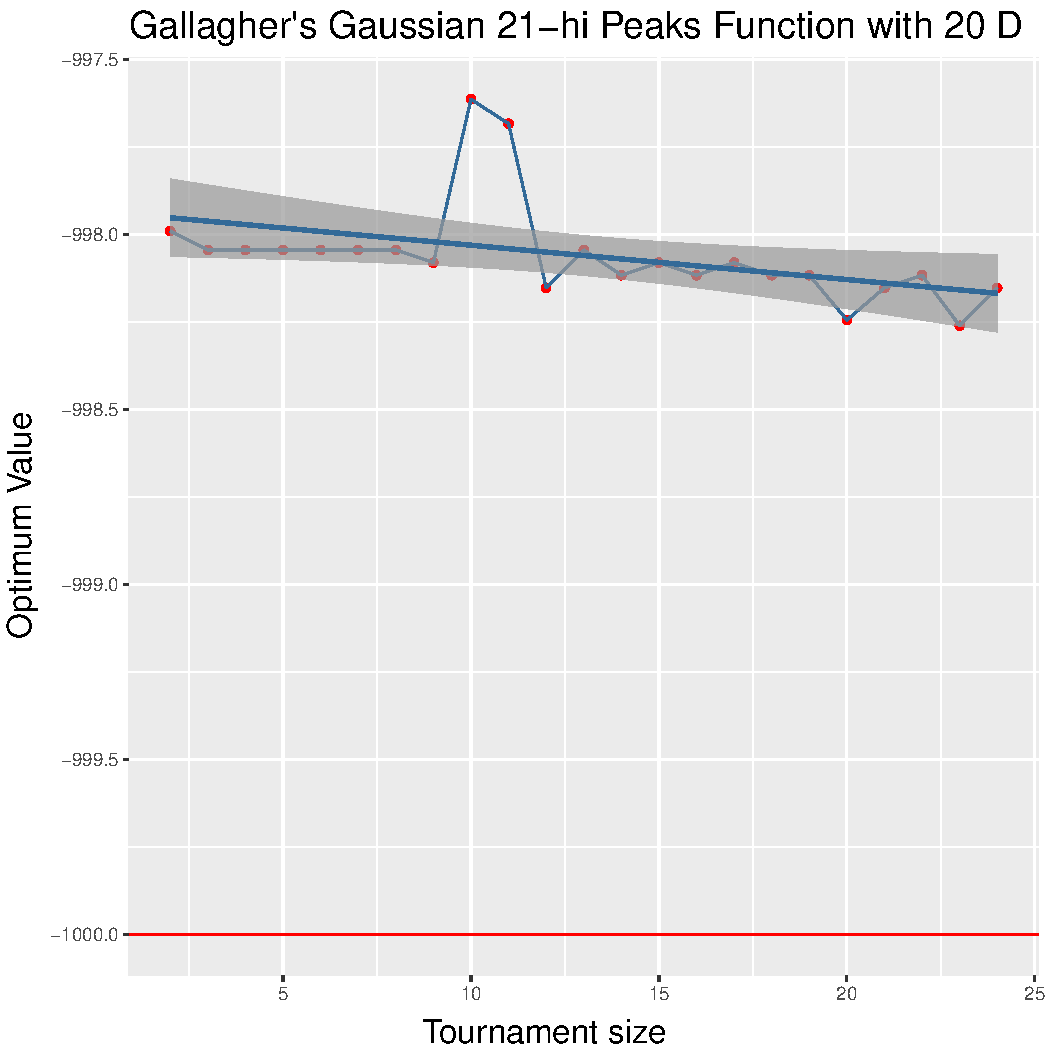
\includegraphics[width=\textwidth]{img/multimodal_sbx_22_dim_20.pdf}
		\caption{10 dimensions.}
	\end{subfigure}
	\begin{subfigure}[b]{0.33\textwidth}
		\centering
		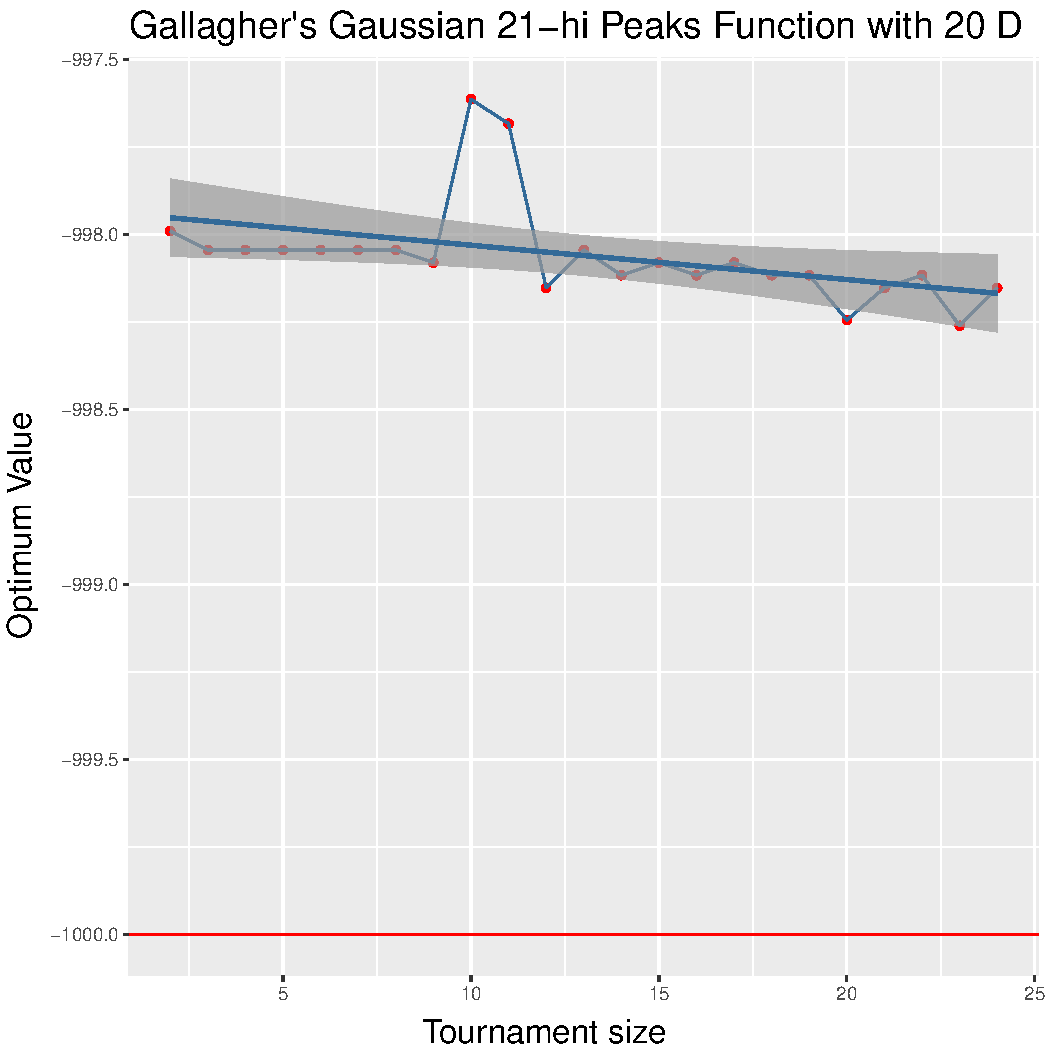
\includegraphics[width=\textwidth]{img/multimodal_sbx_22_dim_20.pdf}
		\caption{20 dimensions.}
	\end{subfigure}
	\begin{subfigure}[b]{0.33\textwidth}
		\centering
		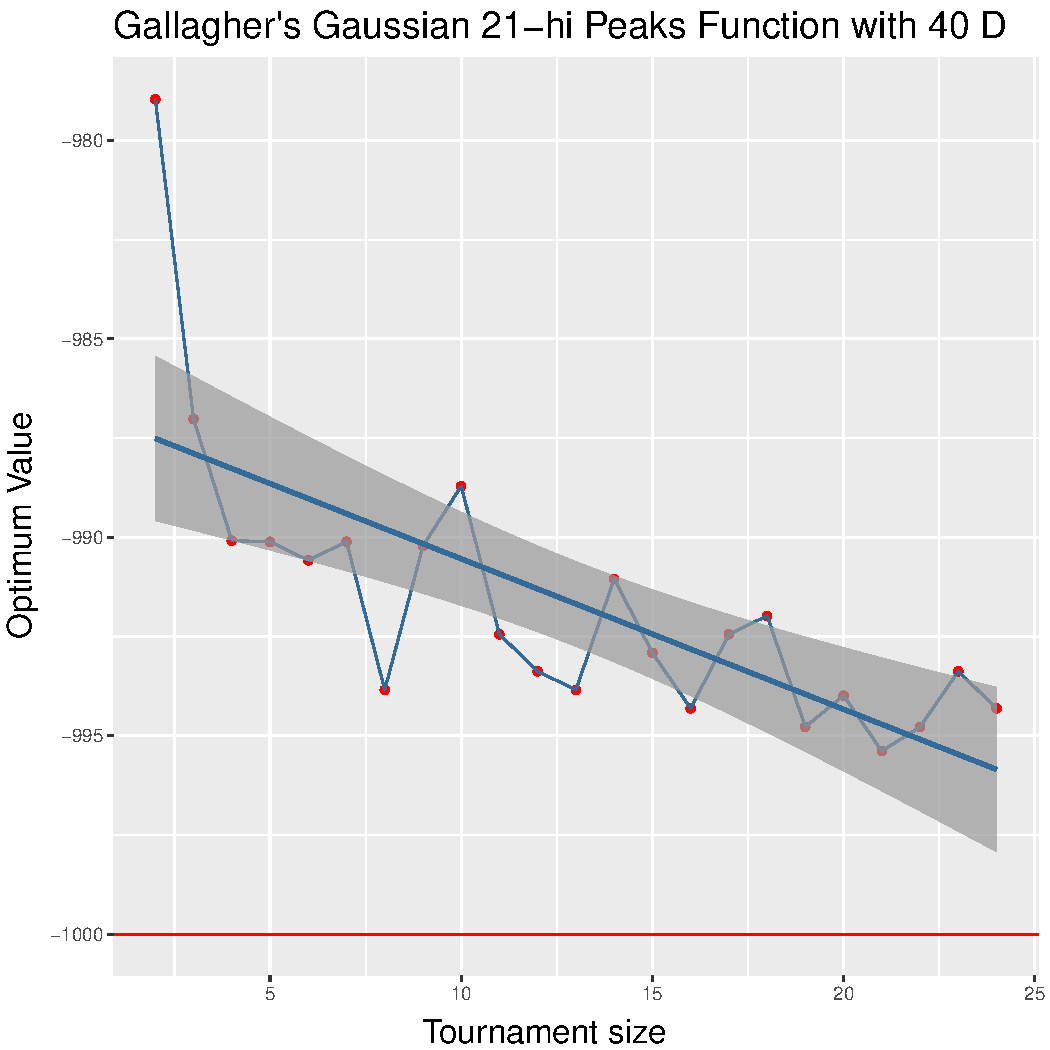
\includegraphics[width=\textwidth]{img/multimodal_sbx_22_dim_40.pdf}
		\caption{40 dimensions.}
	\end{subfigure}
	\caption{Average performance on different tournament size for the Gallagher's Gaussian 21-hi Peaks Function, when using the SBX crossover - Gen. Scheme A.}
	\label{sbx-22}
\end{figure*}

\begin{figure*}[t]
	\begin{subfigure}[b]{0.33\textwidth}
		\centering
		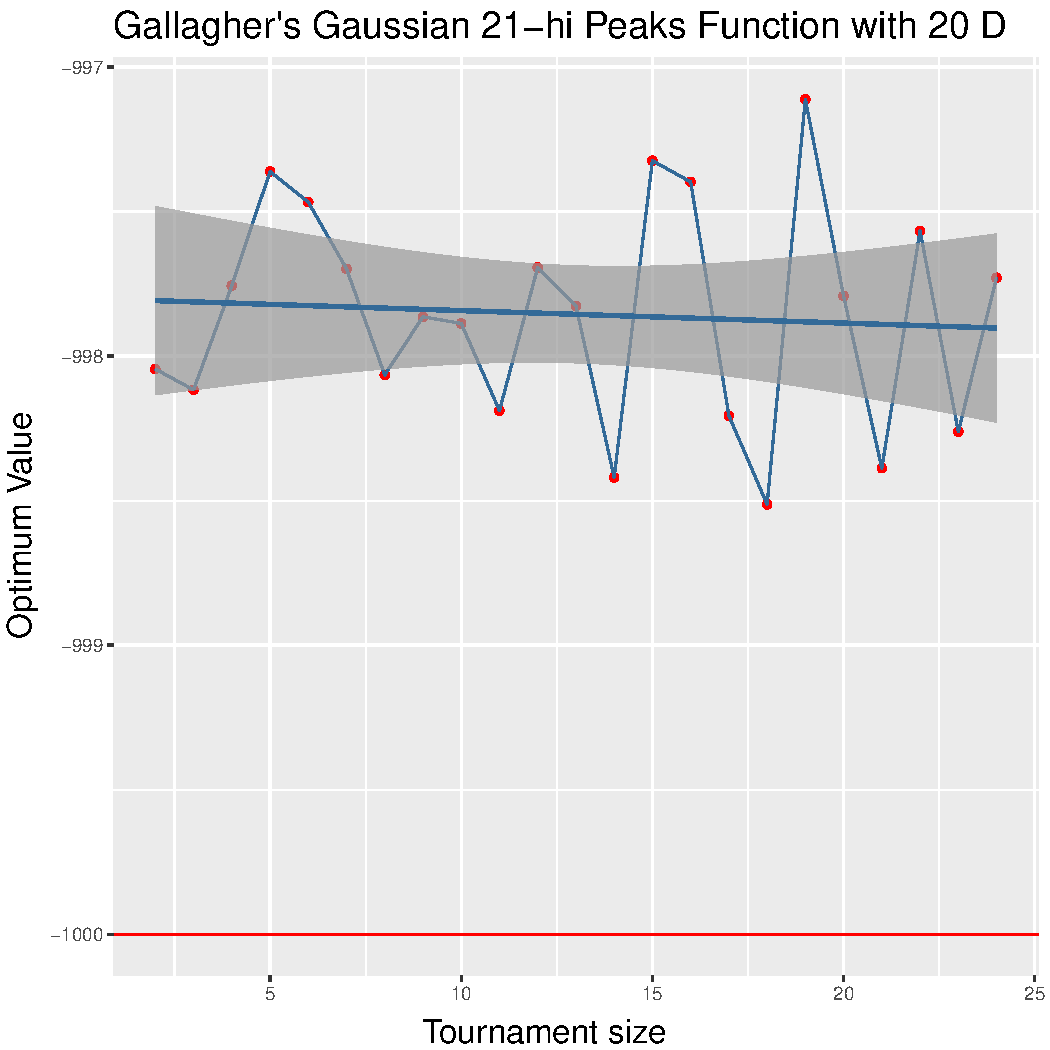
\includegraphics[width=\textwidth]{img/multimodal_uniform_22_dim_20.pdf}
		\caption{10 dimensions.}
	\end{subfigure}
	\begin{subfigure}[b]{0.33\textwidth}
		\centering
		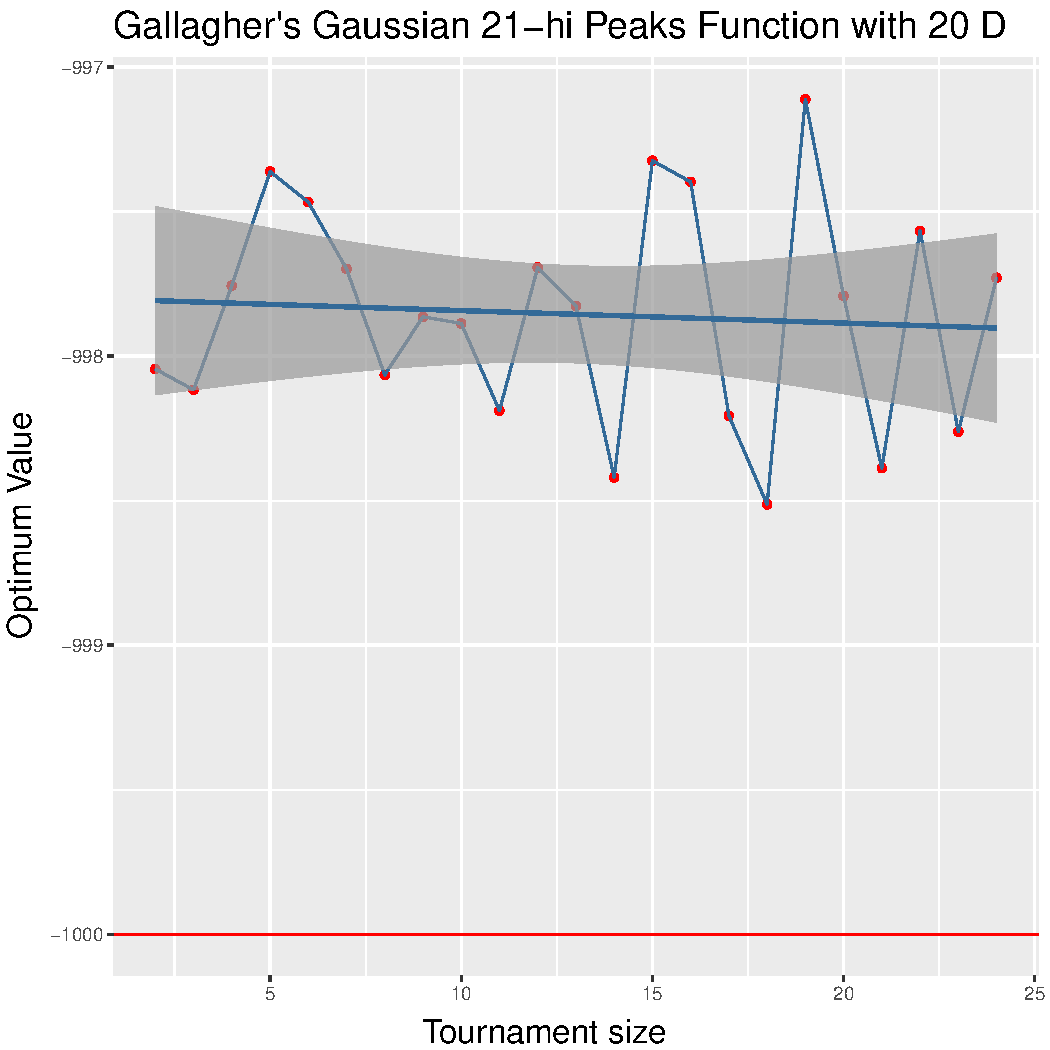
\includegraphics[width=\textwidth]{img/multimodal_uniform_22_dim_20.pdf}
		\caption{20 dimensions.}
	\end{subfigure}
	\begin{subfigure}[b]{0.33\textwidth}
		\centering
		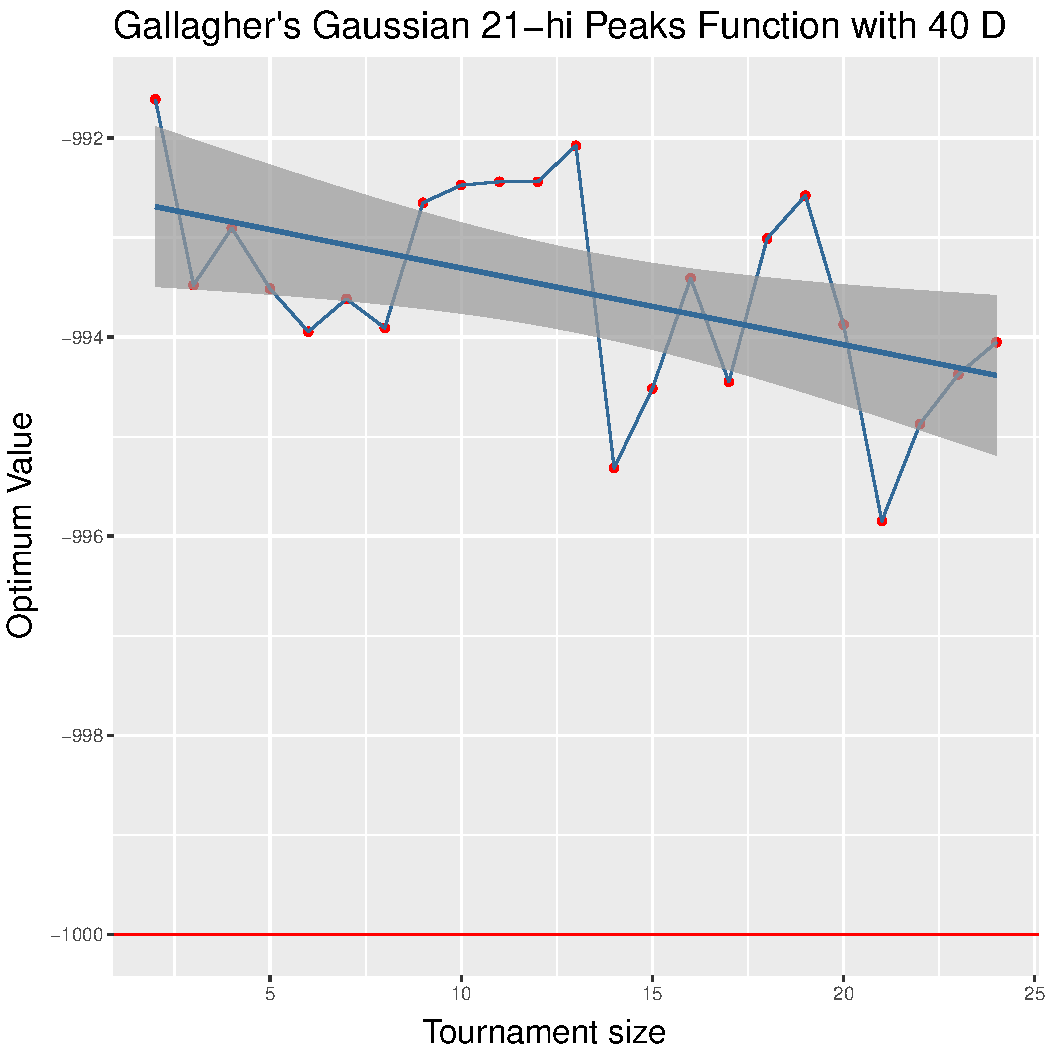
\includegraphics[width=\textwidth]{img/multimodal_uniform_22_dim_40.pdf}
		\caption{40 dimensions.}
	\end{subfigure}
	\caption{Average performance on different tournament size for the Gallagher's Gaussian 21-hi Peaks Function, when using the uniform crossover - Gen. Scheme A.}
	\label{uniform-22}
\end{figure*}

\begin{figure*}[t]
	\begin{subfigure}[b]{0.33\textwidth}
		\centering
		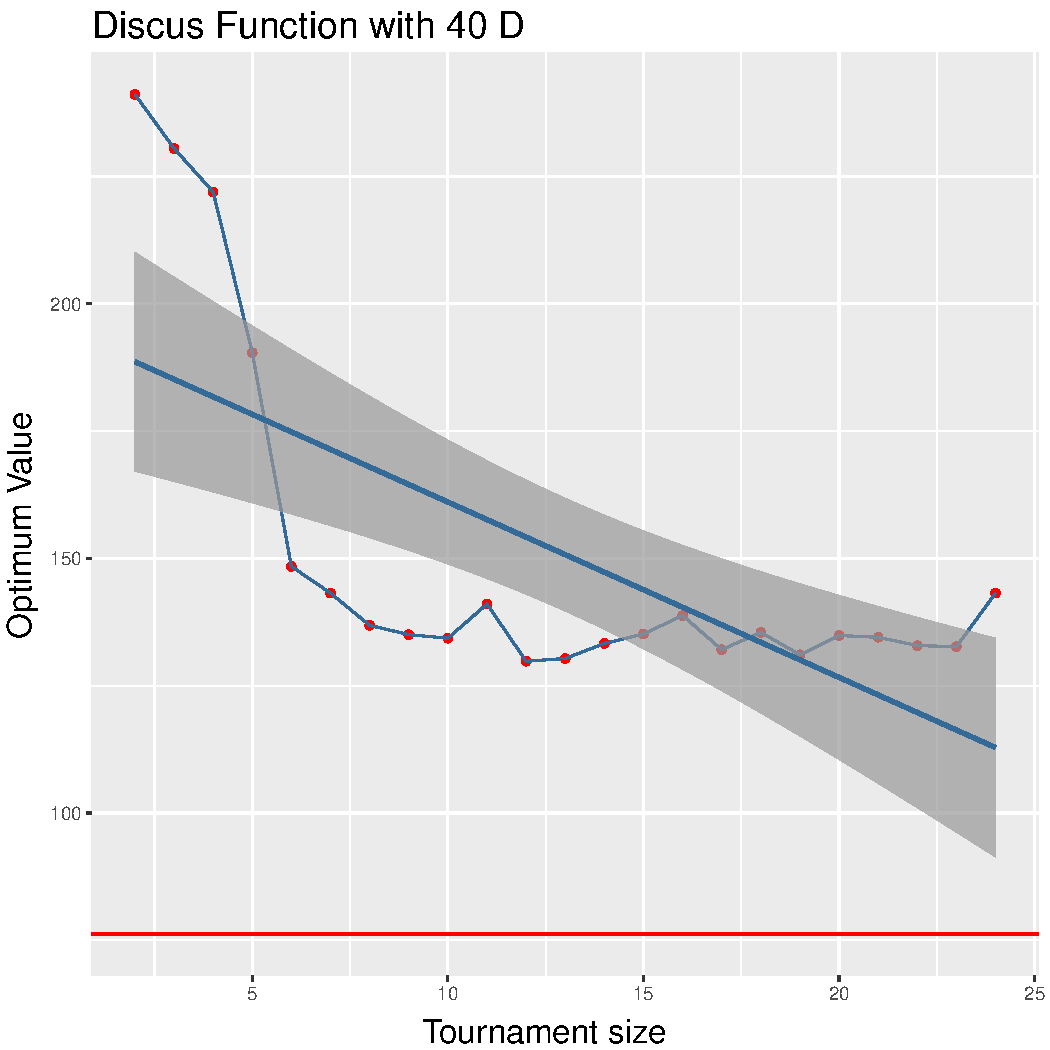
\includegraphics[width=\textwidth]{img/unimodal_sbx_11_dim_40.pdf}
		\caption{10 dimensions.}
	\end{subfigure}
	\begin{subfigure}[b]{0.33\textwidth}
		\centering
		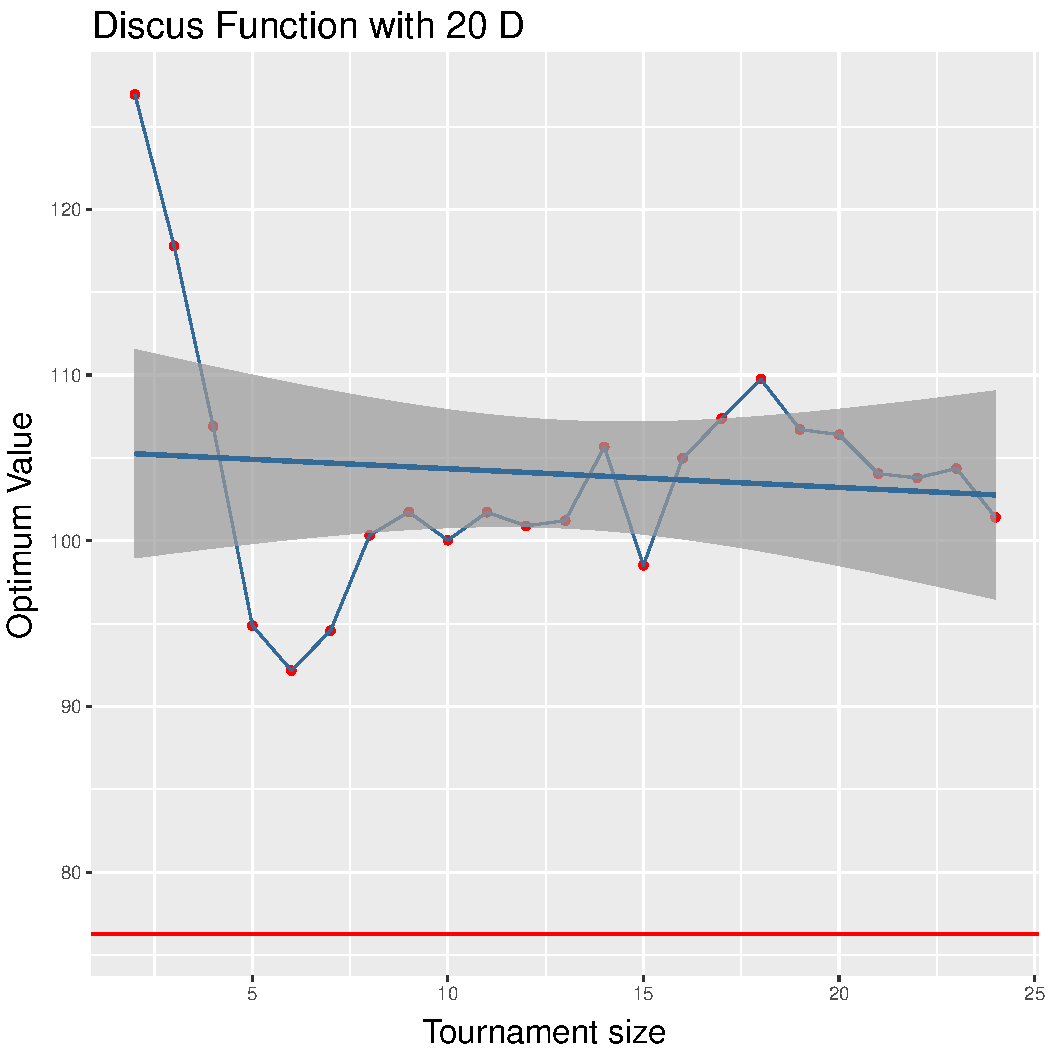
\includegraphics[width=\textwidth]{img/unimodal_sbx_11_dim_20.pdf}
		\caption{20 dimensions.}
	\end{subfigure}
	\begin{subfigure}[b]{0.33\textwidth}
		\centering
		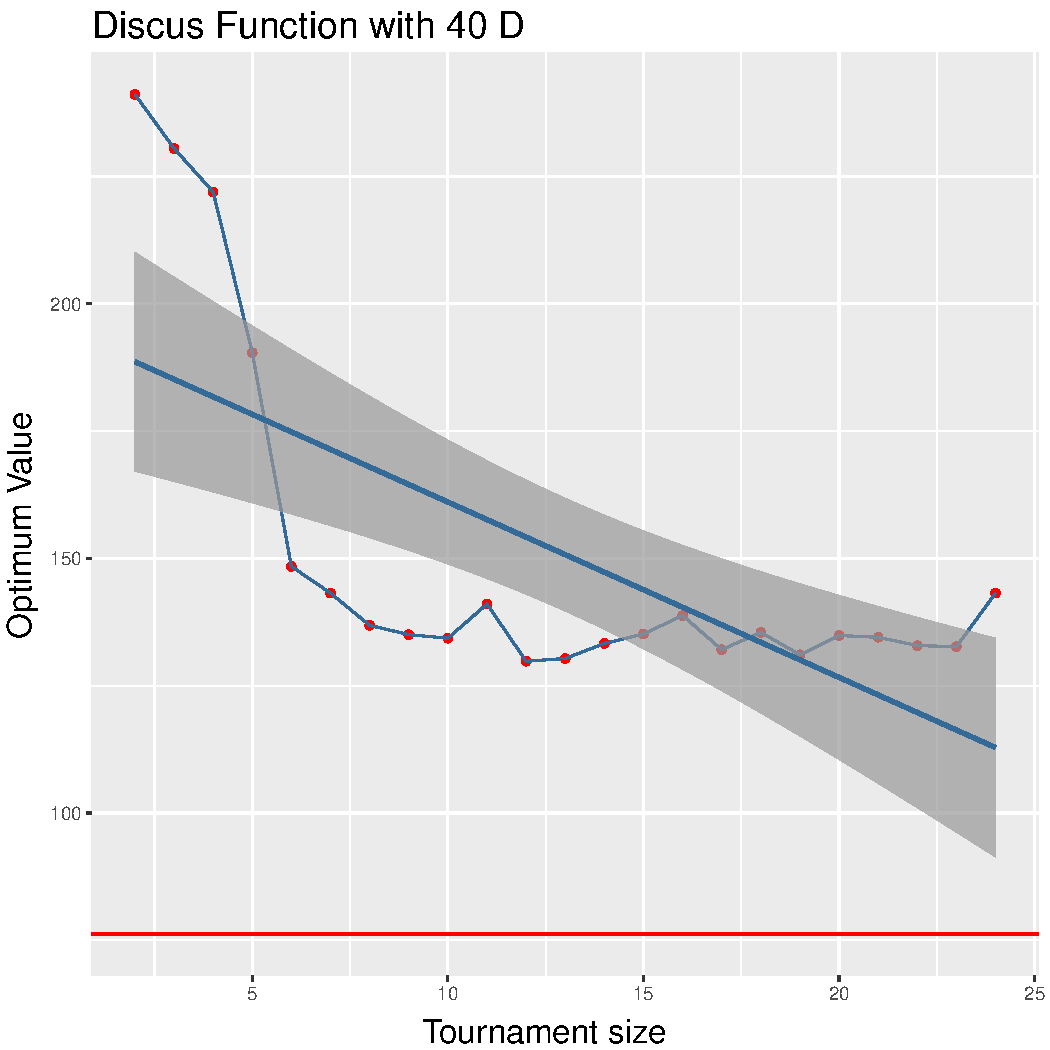
\includegraphics[width=\textwidth]{img/unimodal_sbx_11_dim_40.pdf}
		\caption{40 dimensions.}
	\end{subfigure}
	\caption{Average performance on different tournament size for the Discus Function, when using the SBX crossover - Gen. Scheme A.}
	\label{sbx-11}
\end{figure*}


\begin{figure*}[t]
	\begin{subfigure}[b]{0.33\textwidth}
		\centering
		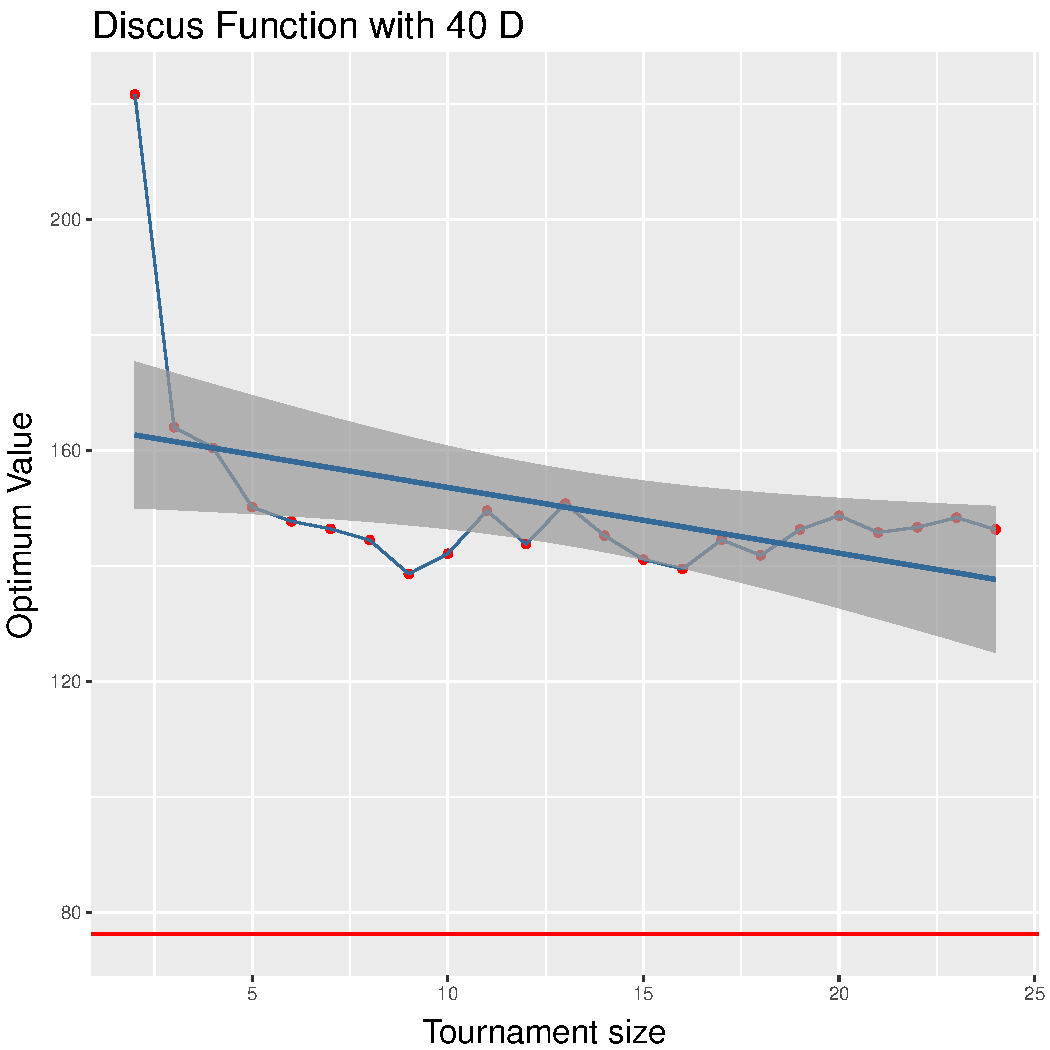
\includegraphics[width=\textwidth]{img/unimodal_uniform_11_dim_40.pdf}
		\caption{10 dimensions.}
	\end{subfigure}
	\begin{subfigure}[b]{0.33\textwidth}
		\centering
		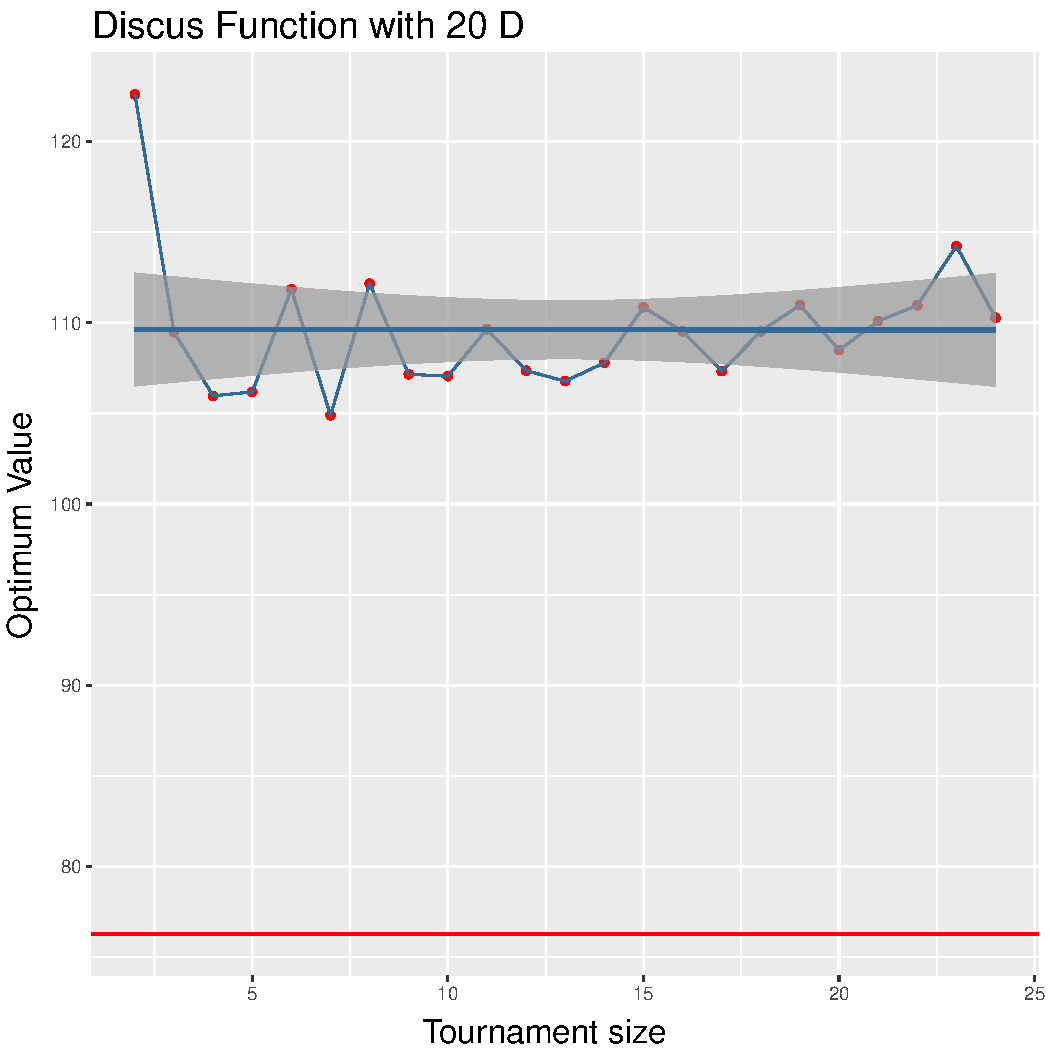
\includegraphics[width=\textwidth]{img/unimodal_uniform_11_dim_20.pdf}
		\caption{20 dimensions.}
	\end{subfigure}
	\begin{subfigure}[b]{0.33\textwidth}
		\centering
		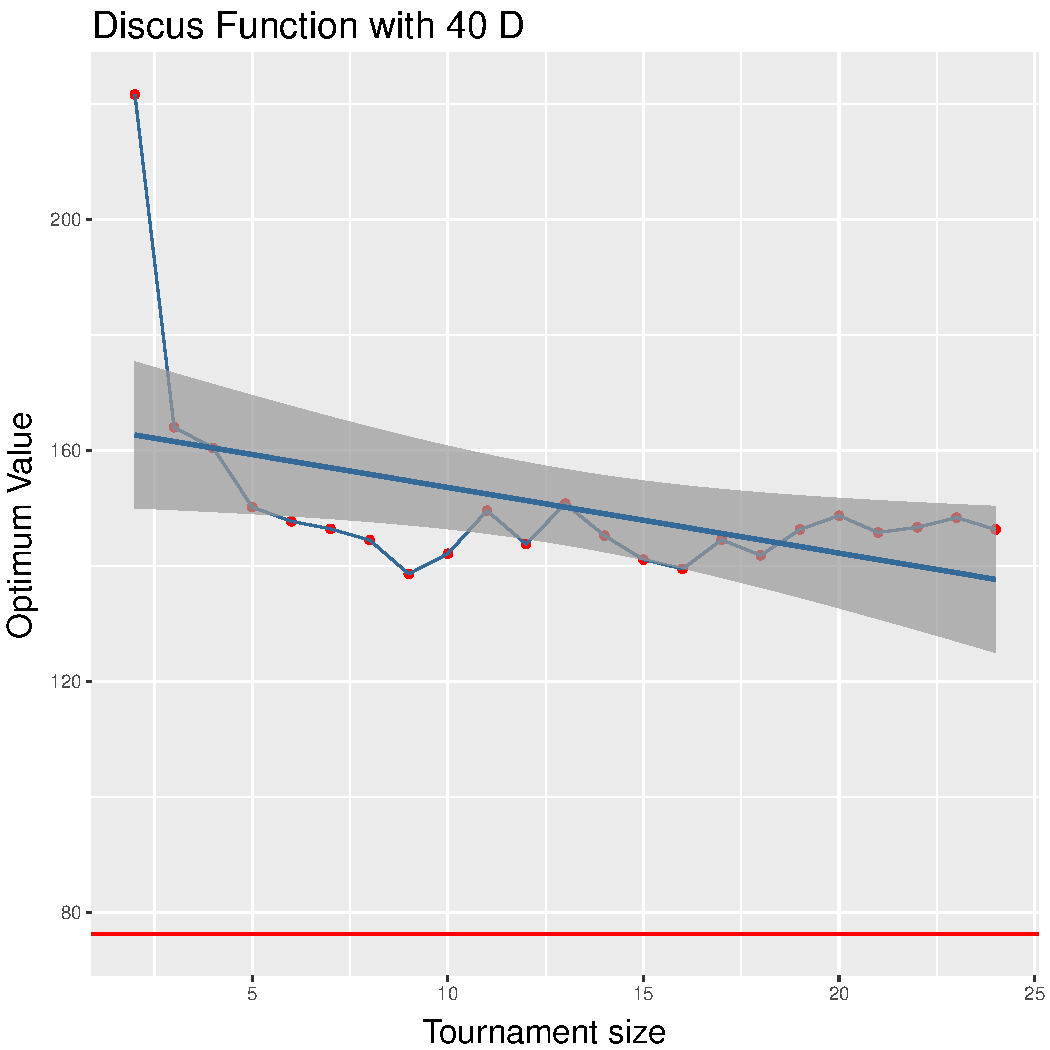
\includegraphics[width=\textwidth]{img/unimodal_uniform_11_dim_40.pdf}
		\caption{40 dimensions.}
	\end{subfigure}
	\caption{Average performance on different tournament size for the Discus Function, when using the uniform crossover - Gen. Scheme A.}
	\label{uniform-11}
\end{figure*}


To get a finer intuition about the results, we show  some visual examples, separated in two groups of Figures. The first group, shows the mean value achieved by the GA given a function. The second one, shows the convergence plot with the mean of the values found at each generation, the function target value with a given tournament size. All Figures represent the mean of 34 repetitions given a certain dimension.



\subsection{Tournament Size by Functions Analysis}
The Figures~\ref{sbx-22} and ~\ref{uniform-22} exemplify that for the Gallagher's Gaussian 21-hi Peaks Function (with 10, 20 and 40 dimensions) changing the tournament size for higher values tend to increase the quality of the results, with greater variation when the SBX crossovers, Figure~\ref{sbx-22}, in used when comparing with the uniform crossover. Figure~\ref{uniform-22}.

For the Discus Function, the Figures~\ref{sbx-11},~\ref{uniform-11}, (with 10, 20 and 40 dimensions) show that the same trend is observed. 

The gray shaded area represents the 95\% confidence level interval for predictions from a linear model for each scenario showed and demonstrate that choosing small values for the tournament size, as 2 or 3 can be a very poor choice. For all Figures, the mean of 34 repetitions is shown as bullets and the red line is shows the objective target value for the function.


\subsection{Convergence Analysis}
The Figures~\ref{convegence-11} and~\ref{convergence-23} exemplify that for the Discus Function with 40 dimensions and with the SBX crossover the GA is converging towards the optimum target value, represented by the bottom, red, horizontal line. The same convergence is observed with the uniform crossover for the Katsuura Function. We found similar behavior in most of the functions, given any crossover operator.

\begin{figure}[t]
	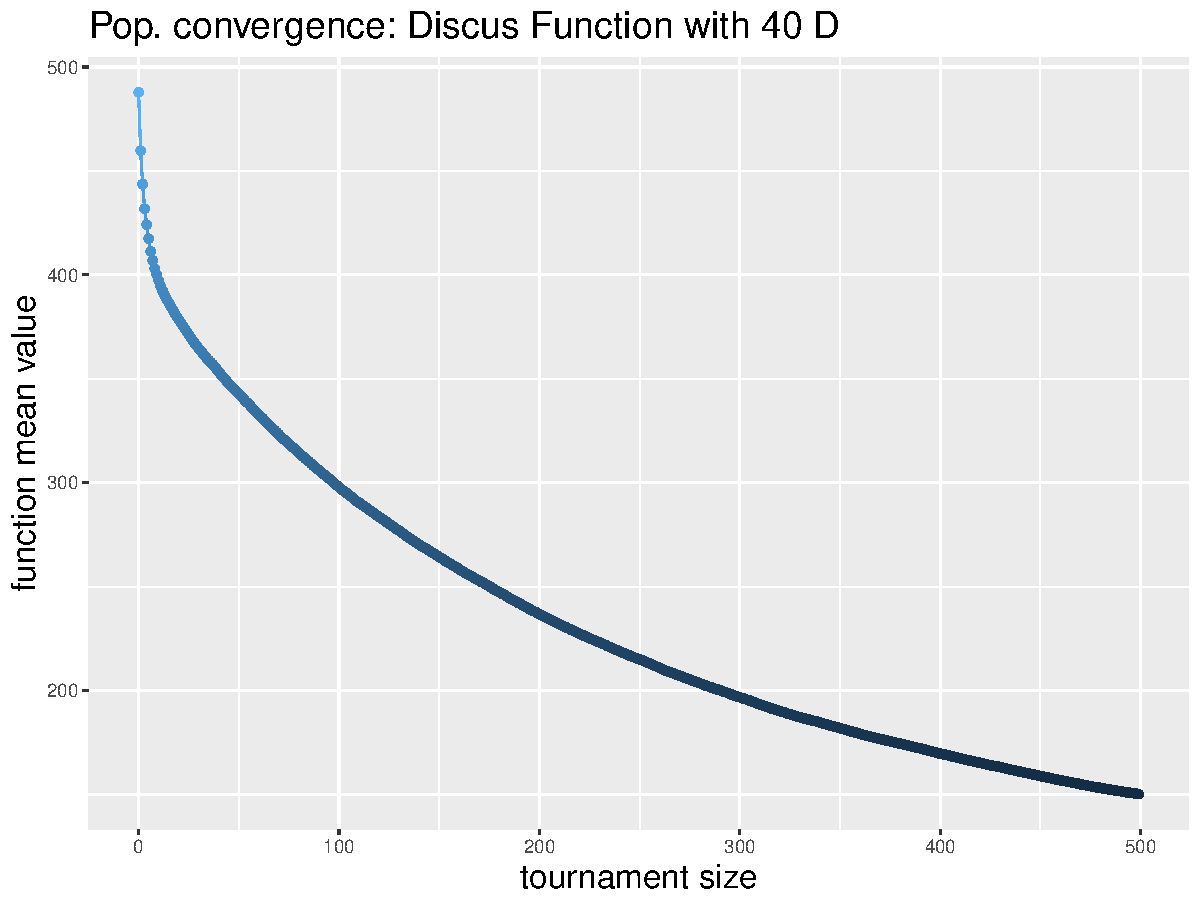
\includegraphics[width=0.5\textwidth]{img/Uniform_convergence_40D_DiscusF.pdf}
	\caption{Population convergence for Discus Function.}
	\label{convegence-11}
\end{figure}


\begin{figure}[t]
	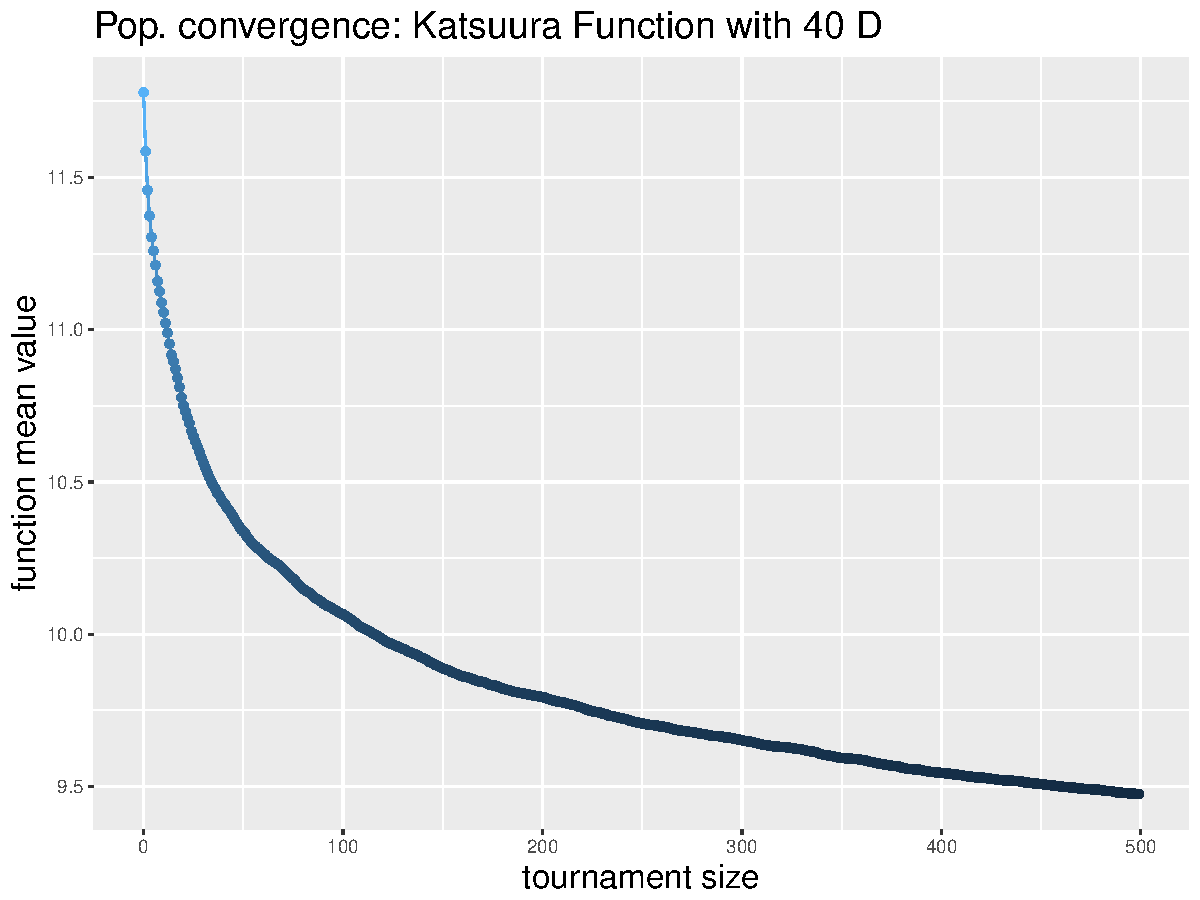
\includegraphics[width=0.5\textwidth]{img/Sbx_convergence_40D_katsuuraF.pdf}
	\caption{Population convergence for Katsuura Function.}
	\label{convergence-23}
\end{figure}


\subsection{Generational Scheme B}


The Friedman Test showed no significant difference in values among tournament size values across all functions, for any configuration, with the SBX crossover. This results hold for every scenario with 40 dimensions, given: all functions (unimodal or multimodal); only the unimodal functions; or only the multimodal functions. 

\begin{table}[h]
	\centering
	\begin{tabular}{|l|l|l|l|}
		\hline
		\textbf{Function Group} & \textbf{Dimension size}      & \textbf{Chi-squared}        & \textbf{P-value}                     \\ \hline
		\multicolumn{1}{|l|}{All} & \multicolumn{1}{|l|}{10} & \multicolumn{1}{l|}{ } & \multicolumn{1}{l|}{ } \\ \hline
		\multicolumn{1}{|l|}{Unimodal} & \multicolumn{1}{|l|}{10} & \multicolumn{1}{l|}{ } & \multicolumn{1}{l|}{ } \\ \hline
		\multicolumn{1}{|l|}{Multimodal} & \multicolumn{1}{|l|}{10} & \multicolumn{1}{l|}{ } & \multicolumn{1}{l|}{ }  \\ \hline
		\hline
		\multicolumn{1}{|l|}{All} & \multicolumn{1}{|l|}{20} & \multicolumn{1}{l|}{ } & \multicolumn{1}{l|}{ } \\ \hline
		\multicolumn{1}{|l|}{Unimodal} & \multicolumn{1}{|l|}{20} & \multicolumn{1}{l|}{ } & \multicolumn{1}{l|}{ } \\ \hline
		\multicolumn{1}{|l|}{Multimodal} & \multicolumn{1}{|l|}{20} & \multicolumn{1}{l|}{ } & \multicolumn{1}{l|}{ }  \\ \hline
		\hline	
		\multicolumn{1}{|l|}{All} & \multicolumn{1}{|l|}{40} & \multicolumn{1}{l|}{27.335} & \multicolumn{1}{l|}{0.1988} 						\\ \hline
		\multicolumn{1}{|l|}{Unimodal} & \multicolumn{1}{|l|}{40} & \multicolumn{1}{l|}{31.111} & \multicolumn{1}{l|}{0.09387} \\ \hline
		\multicolumn{1}{|l|}{Multimodal} & \multicolumn{1}{|l|}{40} & \multicolumn{1}{l|}{25.928} & \multicolumn{1}{l|}{0.2548}  \\ \hline
	\end{tabular}
	\caption{Friedman Test results for SBX Crossover - Gen. Scheme B.}
	\label{Friedman_test_uniform-B}	
\end{table}

As for the generation Scheme A, we show visual examples to get a finer intuition about the results, we show  some visual examples, separated in two groups of Figures. The first group, shows the mean value achieved by the GA given a function. The second one, shows the convergence plot with the mean of the values found at each generation, the function target value with a given tournament size. All Figures represent the mean of 34 repetitions given a certain dimension.


\begin{figure*}[t]
	\begin{subfigure}[b]{0.33\textwidth}
		\centering
		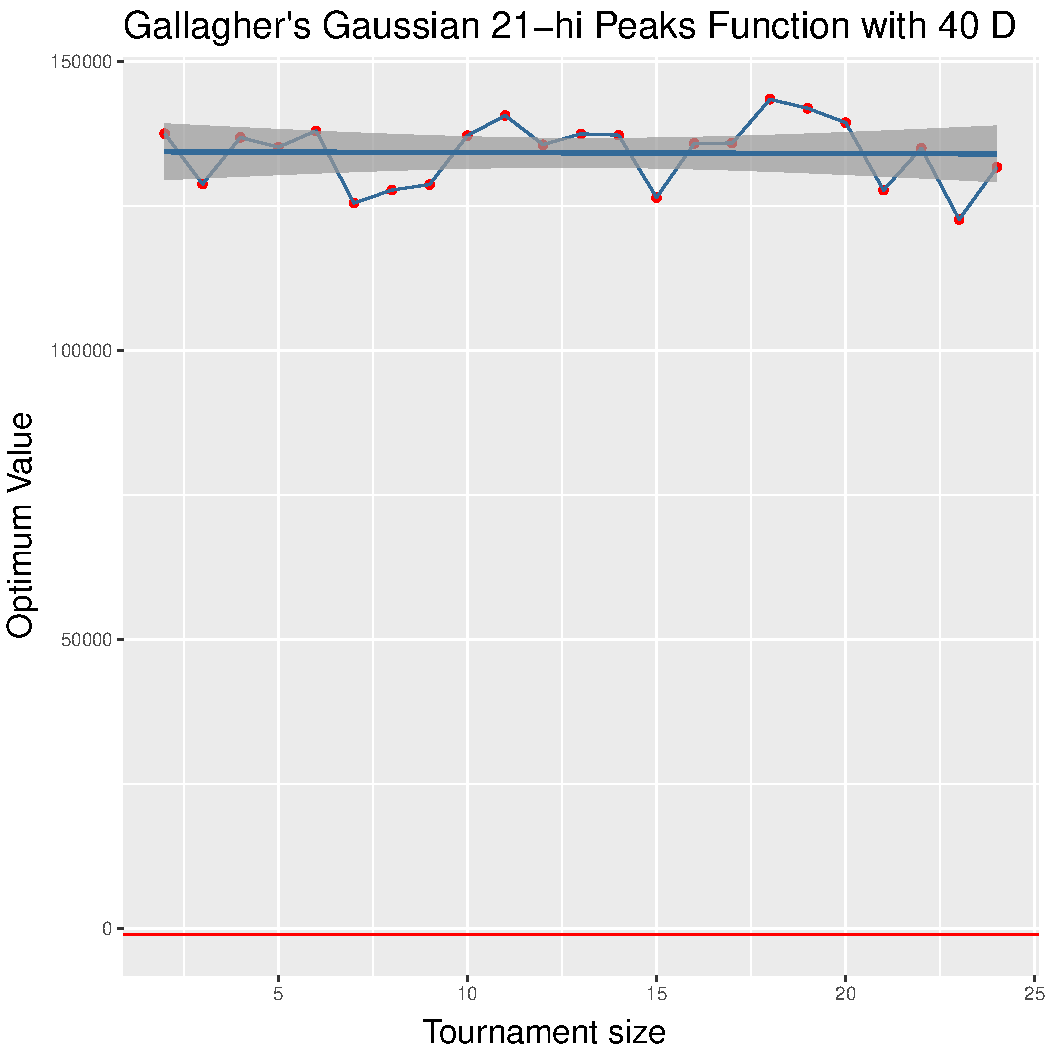
\includegraphics[width=\textwidth]{img/multimodal_2n2n_22_dim_40.pdf}
		\caption{10 dimensions.}
	\end{subfigure}
	\begin{subfigure}[b]{0.33\textwidth}
		\centering
		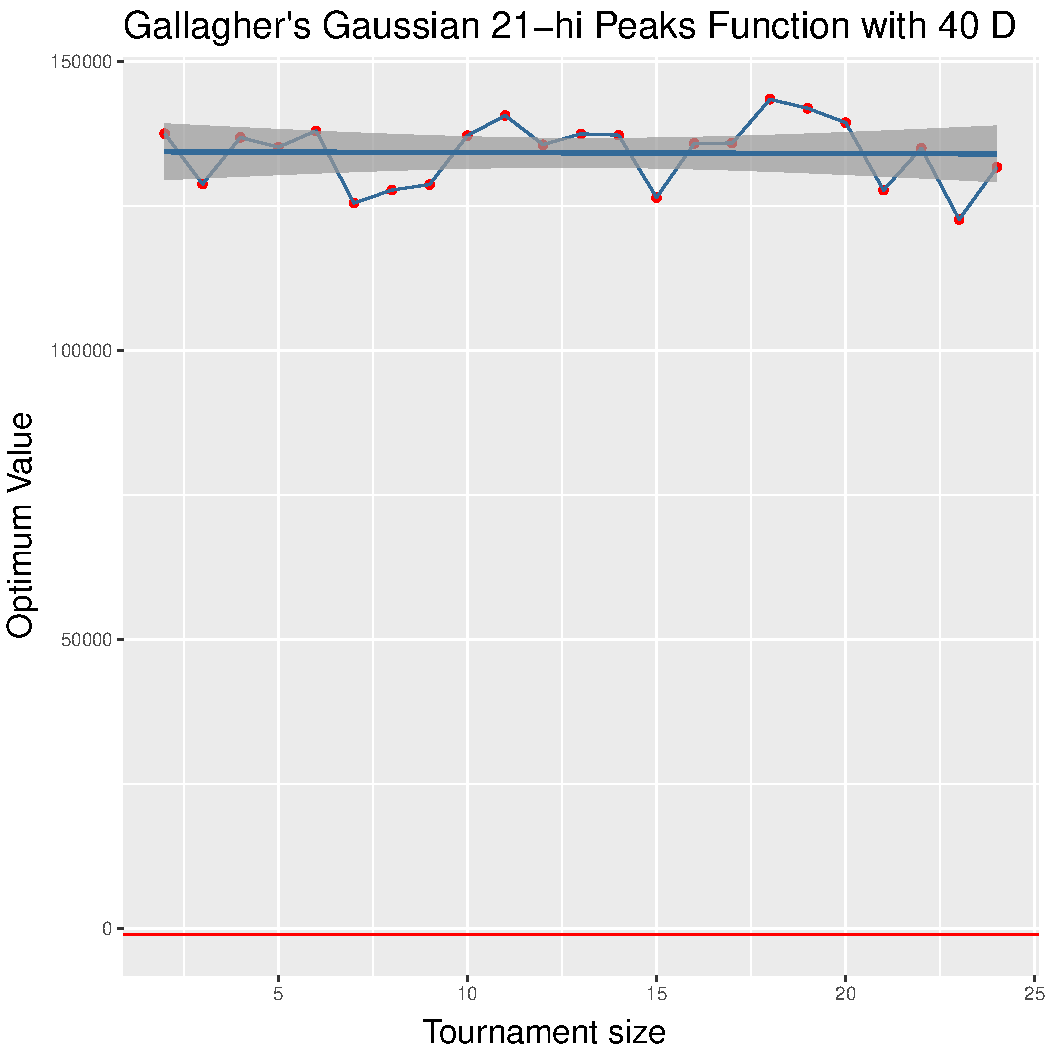
\includegraphics[width=\textwidth]{img/multimodal_2n2n_22_dim_40.pdf}
		\caption{20 dimensions.}
	\end{subfigure}
	\begin{subfigure}[b]{0.33\textwidth}
		\centering
		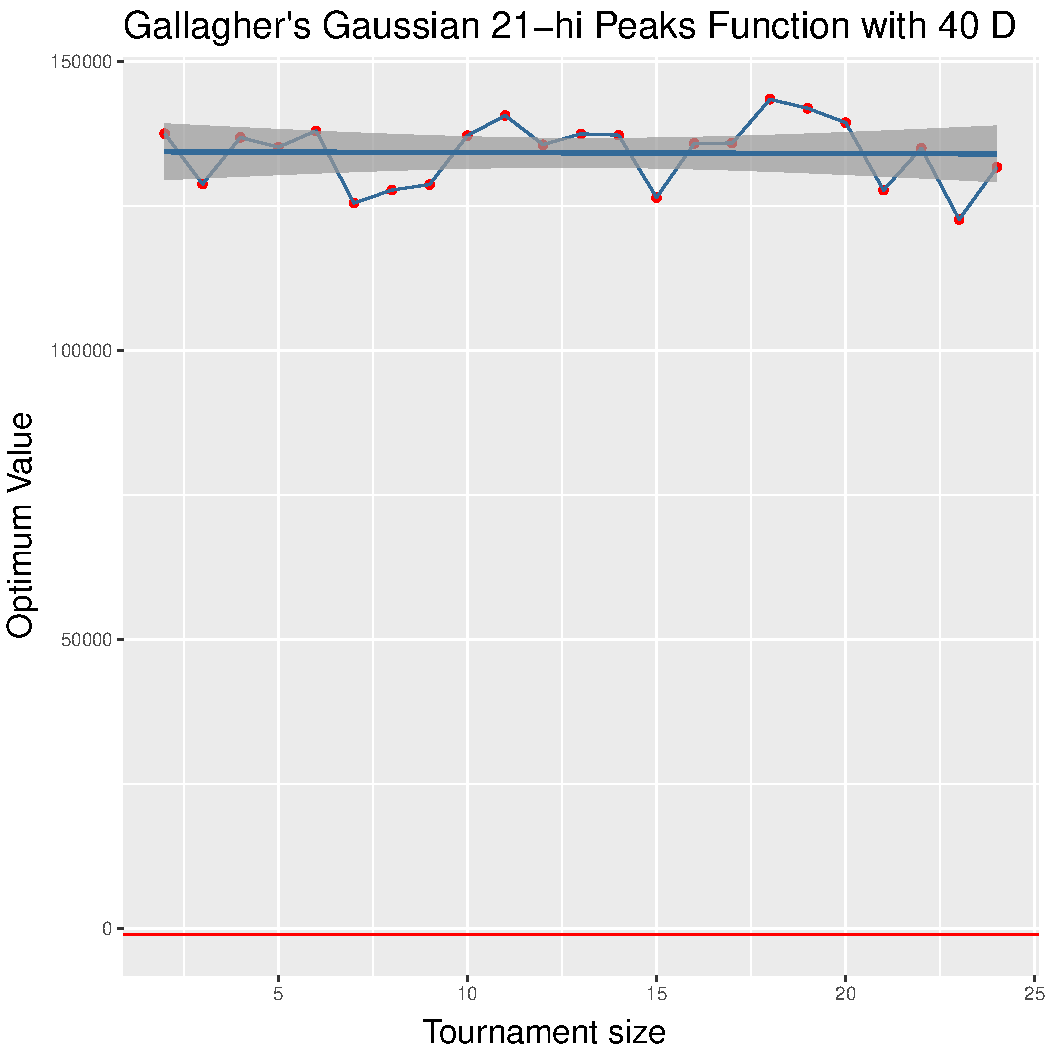
\includegraphics[width=\textwidth]{img/multimodal_2n2n_22_dim_40.pdf}
		\caption{40 dimensions.}
	\end{subfigure}
	\caption{Average performance on different tournament size for the Gallagher's Gaussian 21-hi Peaks Function, when using the SBX crossover - Gen. Scheme B.}
	\label{sbx-22-B}
\end{figure*}

\begin{figure*}[t]
	\begin{subfigure}[b]{0.33\textwidth}
		\centering
		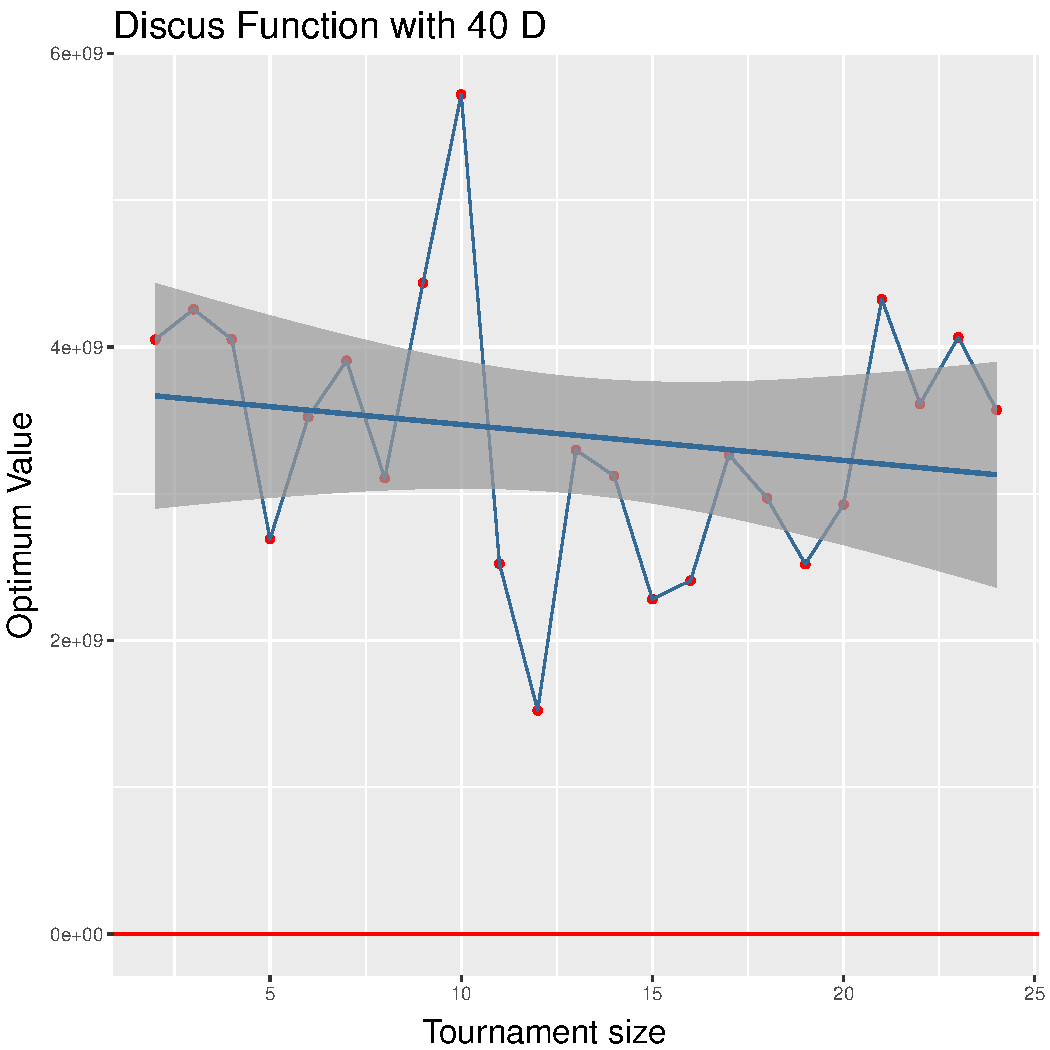
\includegraphics[width=\textwidth]{img/unimodal_2n2n_11_dim_40.pdf}
		\caption{10 dimensions.}
	\end{subfigure}
	\begin{subfigure}[b]{0.33\textwidth}
		\centering
		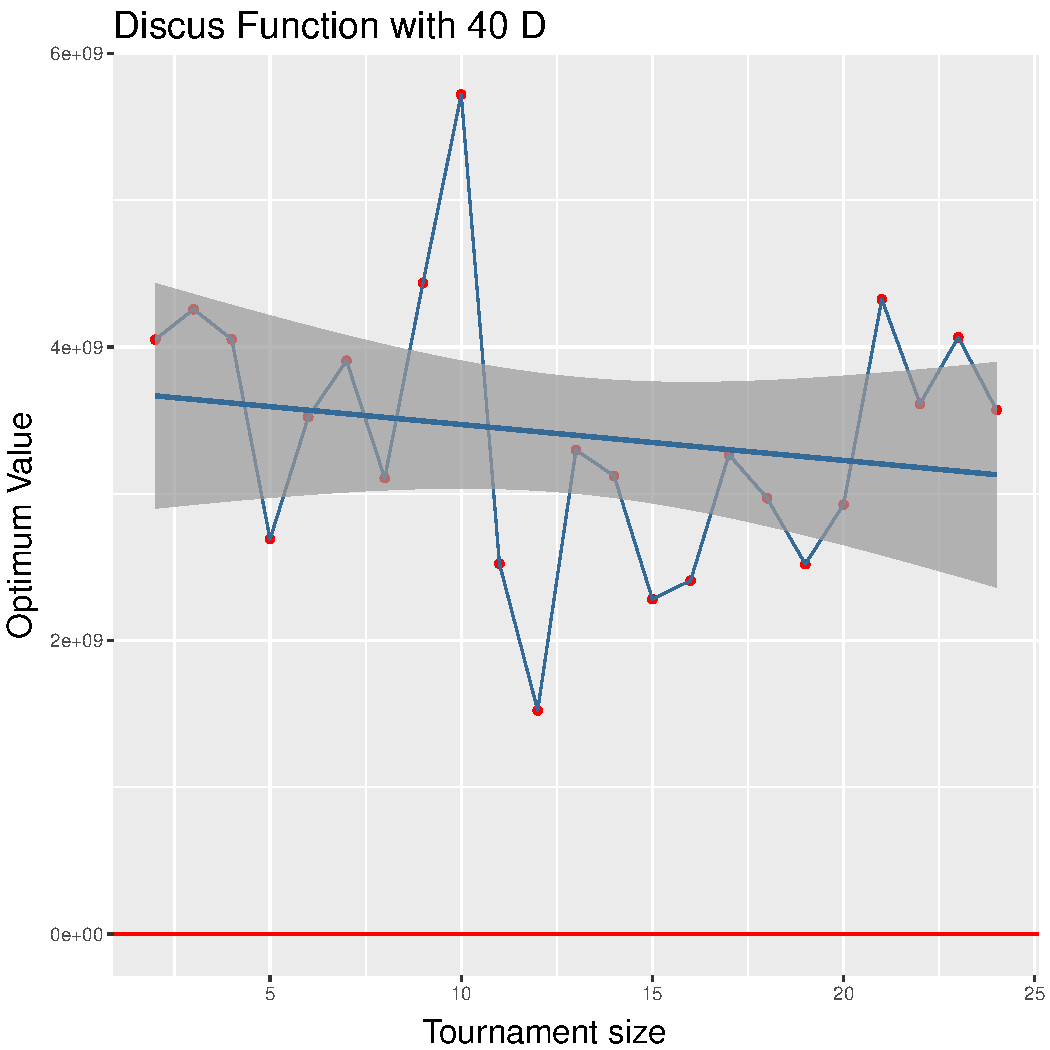
\includegraphics[width=\textwidth]{img/unimodal_2n2n_11_dim_40.pdf}
		\caption{20 dimensions.}
	\end{subfigure}
	\begin{subfigure}[b]{0.33\textwidth}
		\centering
		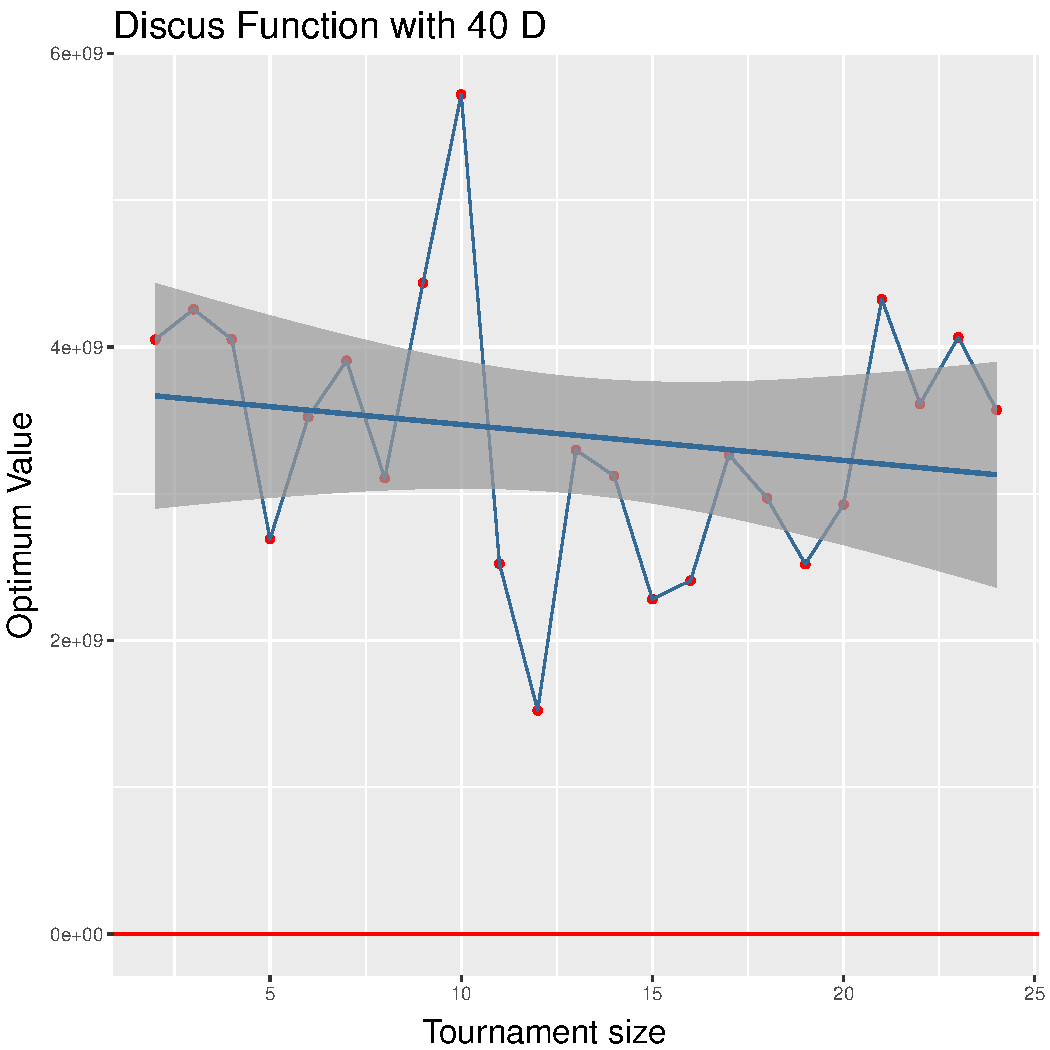
\includegraphics[width=\textwidth]{img/unimodal_2n2n_11_dim_40.pdf}
		\caption{40 dimensions.}
	\end{subfigure}
	\caption{Average performance on different tournament size for the Discus Function, when using the SBX crossover - Gen. Scheme B.}
	\label{sbx-11-B}
\end{figure*}


\subsection{Tournament Size by Functions Analysis}
The Figure~\ref{sbx-22-B} that exemplifies that for the Gallagher's Gaussian 21-hi Peaks Function (with 10, 20 and 40 dimensions) changing the tournament size does not lead to significant better final values found by the GA. The Figure~\ref{sbx-11-B} shows the same trend, but for the Discus Function.

The gray shaded area represents the 95\% confidence level interval for predictions from a linear model for each scenario showed and demonstrate that choosing small values for the tournament size, as 2 or 3 can be a very poor choice. For all Figures, the mean of 34 repetitions is shown as bullets and the red line is shows the objective target value for the function.


\subsection{Convergence Analysis}
The Figures~\ref{convegence-11} and~\ref{convergence-23} exemplify that for the Discus Function with 40 dimensions and with the SBX crossover the GA is converging towards the optimum target value, represented by the bottom, red, horizontal line. The same convergence is observed with the uniform crossover for the Katsuura Function. We found similar behavior in most of the functions, given any crossover operator.
%
%\begin{figure}[t]
%	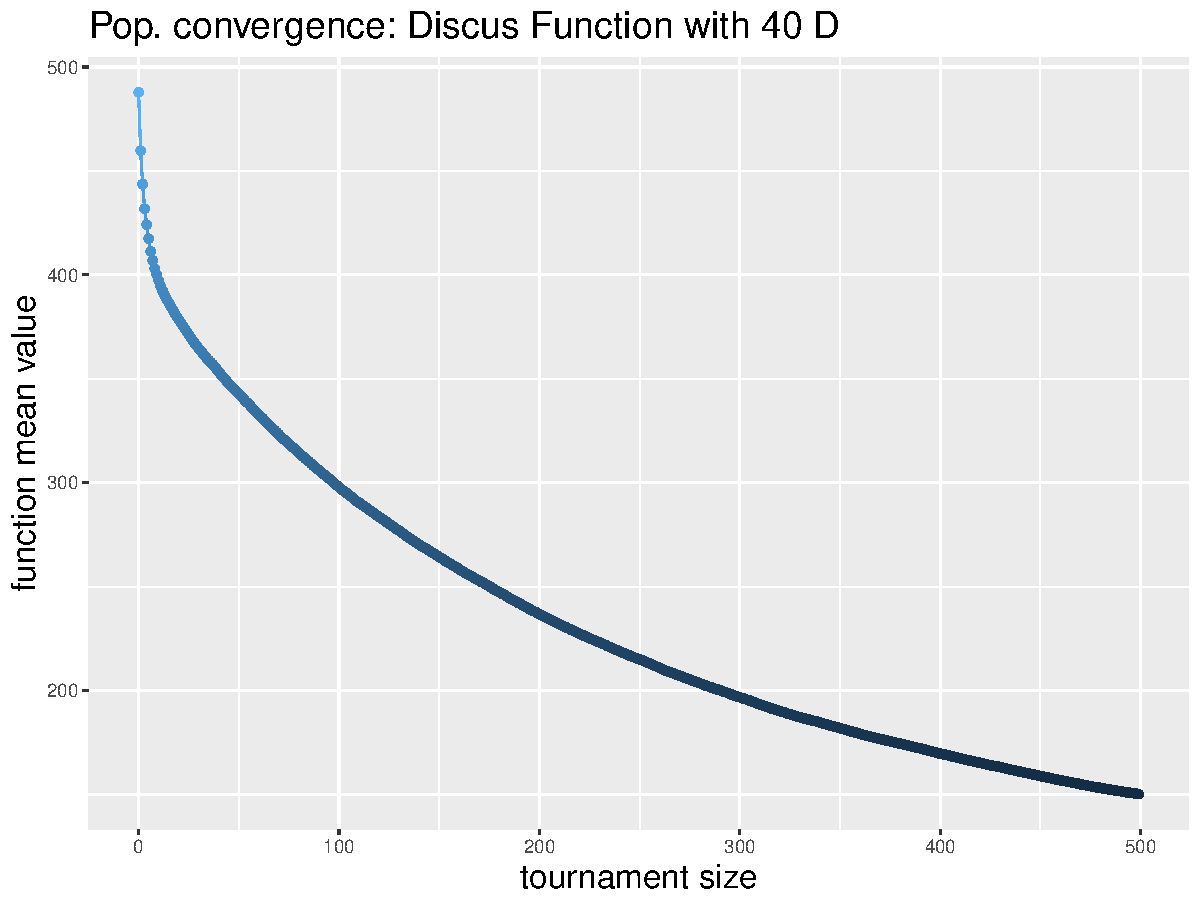
\includegraphics[width=0.5\textwidth]{img/Uniform_convergence_40D_DiscusF.pdf}
%	\caption{Population convergence for Discus Function.}
%	\label{convegence-11}
%\end{figure}

\section{Conclusion}
\label{sec:conclusion}


We proposed an experimental analysis of the impact of the tournament size on the BBOB benchmark functions. We verified that there are little mathematical or experimental studies that supports a choice of value for the tournament size. Usually, the tournament size is chosen to be 2 or 3, based on ``previous results''.
 
 
We analyzed a group of tournament size values on different selection operators and we found that using the tournament size with values like 2 or 3 may not be good choices, depending on the characteristic of the problem you are exploring. For that, we propose that some sort of self-adaptative procedure should be tried, aiming to minimize the impact of bad choice of values for the tournament size.

We are aware that our work is limited to few tournament size values. Also, we understand that the other parameters may have some influence in the results. We know that there is much more that could be done in this field of study, therefore we propose that more investigations need to be done, in order to truly understand the role of the tournament size value related to the quality of final results. Also, we would like to explore whether our results were mainly related with the particular sets of GA operators studied here.


\bibliographystyle{ACM-Reference-Format}
\bibliography{sample-bibliography} 

\end{document}
